% % % % % % % %  MDT UFSM 2021  % % % % % % % % 
%% Arquivo base para o documento - ver. 1.0 %%
% % % % % % % % % % % % % % % % % % % % % % % % 


% % % OPCOES DE COMPILACAO
% % % PAGINACAO
% % % PAGINACAO SIMPLES (FRENTE): PARA TRABALHOS COM MENOS DE 100 PAGINAS
\documentclass[oneside,openright,12pt]{ufsm_2021} %%%%% OPCAO PADRAO -> PAGINACAO SIMPLES. PARA TRABALHOS COM MAIS DE 100 PAGINAS COMENTE ESTA LINHA E DESCOMENTE A LINHA 
% % % % % % % % % % % % % % % % % % % % % % % % % % % % % % % % % % % % % % %
% PAGINACAO DUPLA (FRENTE E VERSO): PARA TRABALHOS COM MAIS DE 100 PAGINAS
% \documentclass[twoside,openright,12pt]{ufsm_2021}  %%%% PARA TRABALHOS COM MAIS DE 100 PAGINAS DESCOMENTE AQUI
% % % % % % % % % % % % % % % % % % % % % % % % % % % % % % % % % % % % %




% % % %  CODIFICACAO DO TEXTO 
% % % %  POR PADRAO USA-SE UTF8. PARA APLICAR A CODIFICACAO OESTE EUROPEU (ISO 8859-1) DESCOMENTE A LINHA ABAIXO. ELA ATIVA A OPCAO "latin1" DO PACOTE "inputenc"
% \oesteeuropeu
% % % % % % % % % % % 



% % % % % % % % PACOTES PESSOAIS % % % % % % % %  
\usepackage{lipsum}
\usepackage{quoting}
\usepackage{gensymb}


% % % % % % % % DEFINICOES PESSOAIS % % % % % % % %







% % % % % % % % % % % % % % % % % % % % % % % % % % % % % % % % % % % % % % % % % % % 




% % % % % % % % % % % % % % % % % % % % % % % % % % % % % % % % % 
% % % % % % % % % % % % DADOS DO TRABALHO % % % % % % % % % % % % 
% % % % % % % % % % % % % % % % % % % % % % % % % % % % % % % % % 

% % % % % % % % % % INFORMACOES INSTITUCIONAIS % % % % % % % % % % 


% % CENTRO DE ENSINO DA UFSM
\centroensino{Centro de Tecnologia}  %%% NOME POR EXTENSO
\centroensinosigla{CT}  %%% SIGLA

% % CURSO DA UFSM
\nivelensino{Bacharelado}  %%%%%%% NIVEL DE ENSINO 
\curso{Engenharia Aeroespacial}   %%%%% NOME POR EXTENSO
\ppg{EA}   %%%%%% SIGLA
\statuscurso{Curso}  %%%% STATUS= {Programa} ou {Curso}
% \EAD  %%%% para cursos EAD
% % % %  LOCAL DO CAMPUS OU POLO
\cidade{Santa Maria}
\estado{RS}


% % % % % % % % % % INFORMACOES DO AUTOR % % % % % % % % % % 
\author{Augusto Pozzebon, Lucas Lira Sassett, Luiz Henrique Schaffazick, Mathias Diettrich}   %%%%% AUTOR DO TRABALHO
\sexo{M} %%%% SEXO DO AUTOR -> M=masculino   F=feminino (IMPORTANTE PARA AJUSTAR PAGINAS PRE-TEXTUAIS)
\grauensino{Bacharel}    %%%%%%%% GRAU DE ENSINO A SER CONCLUIDO
\grauobtido{Bacharelado}    %%%%% TITULO OBTIDO
%\email{lalala@uhul.com}   %%%% E-MAIL PARA CATALOGRAFICA (COPYRIGHT) - OBRIGATORIO
%\endereco{Rua das abobrinhas, n. 666} %%%% TELEFONE PARA CATALOGRAFICA (COPYRIGHT) (CAMPO OPICIONAL -- CASO NAO POSSUA OU NAO QUEIRA DIVULGAR COMENTE A LINHA)
%\fone{11 2222 3333}   %%%% TELEFONE PARA CATALOGRAFICA (COPYRIGHT) FORMATO {11 2222 3333} (CAMPO OPICIONAL -- CASO NAO POSSUA OU NAO QUEIRA DIVULGAR COMENTE A LINHA)
%\fax{11 2222 3333}   %%%% FAX PARA CATALOGRAFICA (COPYRIGHT) FORMATO {11 2222 3333} (CAMPO OPICIONAL -- CASO NAO POSSUA OU NAO QUEIRA DIVULGAR COMENTE A LINHA)


% % % % % % % % % % INFORMACOES DA BANCA % % % % % % % % % % 
% OBSERVACOES: O CAMPO ORIENTADOR EH OBRIGATORIO E NAO DEVE SER COMENTADO
% % % % % %    OS DEMAIS MEMBROS DA BANCA (COOREIENTADOR E DEMAIS PROFESSORES) QUANDO COMENTADOS NAO APARECEM NA FOLHA DE APROVACAO (O LAYOUT DA FOLHA DE APROVACAO ESTA PREPARADO PARA O ORIENTADOR E ATE MAIS 4 MEMBROS NA BANCA
\orientador{André Luis da Silva}{Dr}{AAAA}{M}{P}  %%%INFORMACOES SOBRE ORIENTADOR: OS CAMPOS SAO:{NOME}{SIGLA DA TITULACAO}{SIGLA DA INSTITUICAO DE ORIGEM}{SEXO} M=masculino   F=feminino {PARTE DA BANCA?} P=presidente  M=Membro  N=Nao faz parte
%\coorientador{Maria da Costa}{Dra}{AAAA}{F}{M} %%%INFORMACOES SOBRE CO-ORIENTADOR: OS CAMPOS SAO:{NOME}{SIGLA DA TITULACAO}{SIGLA DA INSTITUICAO DE ORIGEM}{SEXO} M=masculino   F=feminino {PARTE DA BANCA?} P=presidente  M=Membro  N=Nao faz parte
%\bancaum{Banca Um}{Dr}{AAAA}{F}{M}  %%%INFORMACOES SOBRE PRIMEIRO NOME DA BANCA: OS CAMPOS SAO:{NOME}{SIGLA DA TITULACAO}{SIGLA DA INSTITUICAO DE ORIGEM}{SEXO} M=masculino   F=feminino {PARTE DA BANCA?} P=presidente  M=Membro  N=Nao faz parte
%\bancadois{Banca Dois}{Dr}{BBBB}  %%%INFORMACOES SOBRE SEGUNDO NOME DA BANCA: OS CAMPOS SAO:{NOME}{SIGLA DA TITULACAO}{SIGLA DA INSTITUICAO DE ORIGEM}
% \bancatres{Banca Três}{Dra}{CCCC} %%%INFORMACOES SOBRE TERCEIRO NOME DA BANCA: OS CAMPOS SAO:{NOME}{SIGLA DA TITULACAO}{SIGLA DA INSTITUICAO DE ORIGEM}
% \bancaquatro{Banca Quatro}{Dr}{DDDD} %%%INFORMACOES SOBRE QUARTO NOME DA BANCA: OS CAMPOS SAO:{NOME}{SIGLA DA TITULACAO}{SIGLA DA INSTITUICAO DE ORIGEM}
% \bancacinco{Banca Cinco}{Dra}{EEEE} %%%INFORMACOES SOBRE QUARTO NOME DA BANCA: OS CAMPOS SAO:{NOME}{SIGLA DA TITULACAO}{SIGLA DA INSTITUICAO DE ORIGEM}
% \supervisor{Al Paccino}{Dr}{MAFIA}{M}{N} %%%INFORMACOES SOBRE SUPERVISOR (indicado para estagios): OS CAMPOS SAO:{NOME}{SIGLA DA TITULACAO}{SIGLA DA INSTITUICAO DE ORIGEM}{SEXO} M=masculino   F=feminino {PARTE DA BANCA?} P=Presidente  M=Membro  N=Nao faz parte



% % % % % % % % % % REALIZACAO POR VIDEO CONFERENCIA (MEMORANDO 04/2016 BIBLIOTECA CENTRAL UFSM)
%\videoconferencia % % % % QUANDO O ACADEMICO DEFENDE POR VIDEO CONFERENCIA (PERMITIDO PELO ARTIGO 82 DO REGIMENTO GERAL DA PRPGP/UFSM). PARA DEFESAS NAS QUAIS O ACADEMICO ESTA PRESENTE COMENTE ESTA LINHA
% % % % QUANDO UM DOS MEMBROS DA BANCA PARTICIPA POR VIDEO CONFERENCIA INDICAR O MEMBRO DE ACORDO COM A LISTA ABAIXO. CASO CONTRARIO MANTER A PALAVRA "NAO". SAO PERMITIDOS, PELO REGIMENTO PRGPGP (ARTIGO 83) ATE 2 MEMBROS 
%\videoconferenciabancap{NAO}  %%%% PRIMEIRO MEMBRO
%\videoconferenciabancas{NAO}  %%%%% SEGUNDO MEMBRO
% % O > ORIENTADOR
% % CO > COORIENTADOR% % % % QUANDO UM DOS MEMBROS DA BANCA PARTICIPA POR VIDEO CONFERENCIA INDICAR O MEMBRO DE ACORDO COM A LISTA ABAIXO. CASO CONTRARIO MANTER A PALAVRA "NAO". SAO PERMITIDOS, PELO REGIMENTO PRGPGP ATE 2 MEMBROS.
% % 1 > BANCA UM
% % 2 > BANCA DOIS
% % 3 > BANCA TRÊS
% % 4 > BANCA QUATRO
% % 5 > BANCA CINCO
% % S > SUPERVISOR
% % % % % % % % % % % % % % % % % % % % % % % % % % % % % % % % % % % % 



% % % % % % % % % % INFORMACOES SOBRE O TRABALHO % % % % % % % % % %
% % % %  TITULO E SUBTITULO DO TRABALHO: ELES NÃO DEVEM ULTRAPASSAR, JUNTOS, 3 LINHAS NA COMPILAÇÃO DA CAPA. 
% SE O TRABALHO POSSUI SUBTITULO, ADICIONE ':' DENTRO DAS CHAVES ABAIXO 
\titulo{Trabalho 2:} %% NAO EH NECESSARIO CAPITALIZAR
% % % %  TITULO DO TRABALHO EM INGLES
% SE O TRABALHO POSSUI SUBTÍTULO, ADICIONE ':' DENTRO DAS CHAVES ABAIXO 
%\englishtitle{Título do trabalho em inglês:}  %% NAO EH NECESSARIO CAPITALIZAR


% % % % O SUBTÍTULO É OPCIONAL, SE NÃO FOR USADO AS LINHAS ABAIXO DEVEM SER COMENTADAS

% SE O TRABALHO POSSUI SUBTÍTULO, ADICIONE ':' DENTRO DAS CHAVES ABAIXO 
\subtitulo{Mecânica de Voo Espacial} %% NAO EH NECESSARIO CAPITALIZAR
% % % %  SUB TITULO DO TRABALHO EM INGLES
%\subenglishtitle{Subtítulo do trabalho em inglês}  %% NAO EH NECESSARIO CAPITALIZAR

% % % AREA DE CONCENTRACAO DO TRABALHO (CNPQ)
%\areaconcentracao{Área de concentração do CNPq}
% % % TIPO DE TRABALHO - MANTER APENAS UMA LINHA DESCOMENTADA
%\tese  %% Tese de <nivel de ensino>
% \qualificacao %% Exame de Qualificação de <nivel de ensino>
% \dissertacao %% Dissertacao de <nivel de ensino>
% \monografia %% Monografia
% \monografiag  %% Monografia (nao exibe area de concentracao)
% \tf  %% Trabalho Final de <nivel de ensino>
% \tfg  %% Trabalho Final de Graduacao (nao exibe area de concentracao)
% \tcc  %% Trabalho de Conclusao de Curso
% \tccg  %% Trabalho de Conclusao de Curso (nao exibe area de concentracao)
% \relatorio  %% Relatório de Estágio (nao exibe area de concentracao)
%  \generico   %%% Alternativa para aqueles cursos que nao recebem o titulo de bacharel ou licenciado. Ex: engenharia, arquitetura, etc... Os campos abaixo tambem devem ser preenchidos
     \tipogenerico{Trabalho Avaliativo}
%     \tipogenericoen{Tipo de trabalho em inglês}
%     \concordagenerico{o}
%     \graugenerico{Engenheiro Eletricista}
% % % DATA DA DEFESA 
\data{13}{07}{2023} %% FORMATO {DD}{MM}{AAAA}



% % % % %  ALGUMAS ENTRADAS PRE-TEXTUAIS
% % % % CASO NAO QUEIRA UTILIZA-LAS COMENTE A LINHA DE COMANDO
% % % EPIGRAFE
%\epigrafe{Winter is coming!}{Família Stark} %ESTRUTURA DE CAMPOS -> {Texto}{Autor}
% % % DEDICATORIA
%\dedicatoria{Aos que virão depois de nós}
% % % %  AGRADECIMENTOS
%\agradecimentos{A mim!}

% % % % %  RESUMO E PALAVRAS CHAVE DO RESUMO - OBRIGATORIO PARA MDT-UFSM
\resumo{
Este trabalho de graduação aborda a complexidade da mecânica do voo espacial, focando na inserção de um CubeSat 8U em órbita geossíncrona. O estudo envolve a adaptação e modelagem de um foguete existente em Python, com ênfase na distribuição ideal de massa entre os estágios do foguete para maximizar o impulso e alcançar a variação de velocidade requerida. A pesquisa analisa detalhadamente o voo ascendente do foguete, avaliando a factibilidade em termos de impulso de velocidade e energia específica, além de abordar aspectos como inserção orbital, parâmetros inerciais e altitude. Também discutimos o voo ascendente em termos de voo balístico e trajetória de rotação gravitacional, ajustes de parâmetros orbitais, e introduzimos o modelo do veículo de inserção orbital e o conceito de rastro planetário. O resultado esperado é um modelo de foguete capaz de simular a inserção orbital de um CubeSat 8U em órbita geossíncrona, demonstrando a extensão e a complexidade do estudo da mecânica do voo espacial.
}
\palavrachave{Mecânica do voo espacial, CubeSat 8U em órbita geossíncrona, Adaptação e modelagem de foguete em Python, Análise de voo ascendente e inserção orbital}
% "... deverão constar, no mínimo, três palavras-chave, iniciadas em
% letras maiúsculas, cada termo separado dos demais por ponto, e
% finalizadas também por ponto." MDT 2012

% % % % %  ABSTRACT E PALAVRAS CHAVE DO RESUMO - OBRIGATORIO PARA MDT-UFSM
%\abstract{
%Write your abstract here! As recomendações do resumo também se aplicam ao abstract. \lipsum[0-1]
%}
%\keywords{Keyword 1. Keyword 2. Keyword 3. (...)}


% % %  ATIVACAO DE LISTAS E PAGINAS ESPECIAIS
% % %  PARA QUE APARECAO NAO NO TEXTO DESCOMENTE A LINHA ABAIXO -> POR PADRAO TODAS ESTAO ATIVIDADAS

% % LISTA DE FIGURAS 
% \semfiguras   %%(QUANDO ATIVIDA NAO EXIBE A LISTA)
% % LISTA DE GRAFICOS 
 \semgraficos   %%(QUANDO ATIVIDA NAO EXIBE A LISTA)
% % LISTA DE ILUSTRACOES 
 \semilustracoes  %%(QUANDO ATIVIDA NAO EXIBE A LISTA)
% % LISTA DE TABELAS 
% \semtabelas   %%(QUANDO ATIVIDA NAO EXIBE A LISTA)
% % LISTA DE QUADROS 
\semquadros   %%(QUANDO ATIVIDA NAO EXIBE A LISTA)
% % LISTA DE APENDICES 
 \semapendices  %%(QUANDO ATIVIDA NAO EXIBE A LISTA)
% LISTA DE ANEXOS 
 \semanexos   %%(QUANDO ATIVIDA NAO EXIBE A LISTA)


% % % %  LISTA DE ABREVIATURAS - AMBIENTE TABULAR
%%%%%%%% para não utilizar comente as linhas abaixo.
% \abreviaturamax{SIGLAMAX} %%%% coloque aqui a maior sigla (indentacao)
% \listadeabreviaturas{
% 	SIGLA1 & Nome Completo da Sigla 1 \\
% 	SIGLA2 & Nome Completo da Sigla 2 \\
% 	SIGLAMAX &	Nome Completo da Sigla MAX \\
% }


% % % %  LISTA DE SIGLAS - AMBIENTE TABULAR
%%%%%%%% para não utilizar comente as linhas abaixo.
% \siglamax{SIGLAMAX} %%%% coloque aqui a maior sigla (indentacao)
% \listadesiglas{
% SIGLA1 & Nome Completo da Sigla 1 \\
% SIGLA2 & Nome Completo da Sigla 2 \\
% SIGLAMAX &	Nome Completo da Sigla MAX \\
% }


% % % %  LISTA DE SIMBOLOS
%%%%%%%% OBS: O espaco entre colchetes \item[] e um ambiente matematico
%%%%%%%% para não utilizar comente as linhas abaixo.
% \simbolomax{(Re)2} %%%% coloque aqui o maior simbolo (indentacao)
% \listadesimbolos{
% \item[u_*]	Escala de velocidade de fricção	
% \item[w_*]	Escala de velocidade convectiva
% \item[(Re)^2]	Maior simbolo da lista
% }


% % % FICHA CATALOGRAFICA
% \semcatalografica  %%%%  (QUANDO ATIVIDA NAO EXIBE A FICHA CATALOGRAFICA NECESSITA DO ARQUIVO DA FICHA: ficha_catalografica.pdf
% % % A FICHA CATALOGRAFICA FORNECIDA PELA UFSM EH UM PDF DO TAMANHO A4
% % % EH POSSIVEL GERA-LA NO SITE http://cascavel.ufsm.br/ficha_catalografica/
% % % OS COMANDOS ABAIXO DEFINEM AS MARGENS PARA CORTAR A FICHA FORNECIDA E COLOCA-LA COMO UMA FIGURA NO DOCUMENTO LATEX
% \margemesquerda{1.9}   %%%% CORTE DE MARGEM ESQUERDA EM CM
% \margemdireita{1.5}   %%%% CORTE DE MARGEM DIREITA EM CM
% \margemsuperior{2.75}  %%%% CORTE DE MARGEM SUPERIOR EM CM
% \margeminferior{2.9} %%%% CORTE DE MARGEM INFERIOR EM CM
% % %  DICA: IMPRIMA UMA COPIA DA FICHA CATALOGRAFICA E FACA A MEDIDA DAS MARGENS!





% % FOLHA DE ERRATA (versao rudimentar...pode ser aprimorado)
% % para não utilizar comente as linhas abaixo.
% % deve ser preenchida como um ambiente tabular de quatro colunas:
% % pagina & linha & onde se le & leia-a se \\
% \errata{
% 10   &    10    & errado   & certo \\
% \hline
% 12    &    5     & errado com um texto mais longo & certo agora com um texto mais longo\\
% \hline
% 13   &    3    & $x^2$   & $2x$\\
% }
% % % % % % % % % % % % % % % % % % % % % % % % % % % % % % % % % % % % % % % % % % % % % % 


% % % % % % % % % % % % % % % % % % % % % % % % % % % % % % % % % % % % % % 
% % % % % % % % % % % %  OPCOES DE FORMATACAO % % % % % % % % % % % % % % %
% % % % % % % % % % % % % % % % % % % % % % % % % % % % % % % % % % % % % % 
% % % CAPITULO: por padrao alinhado a esquerda. Para ativar alinhamento centralizado descomente o comando abaixo

% \centralizado  %%%% <<< centraliza todos os capitulos

% % % % % % % % % % % % % % % % % % % % % % % % % % % % % % % % % % % % % %
% % % FONTES: descomente uma das opcoes. caso nenhuma seja ativada a clase usara a fonte padrao do latex

%% helvetica
\usepackage[scaled]{helvet}
\renewcommand*\familydefault{\sfdefault}

%% arial
% \renewcommand{\rmdefault}{phv} % Arial
% \renewcommand{\sfdefault}{phv} % Arial

%%times
% \usepackage{mathptmx}

% % % % % % % % % % % % % % % % % % % % % % % % % % % % % % % % % % % % % % 
% % % % % % % % % % % % % % % % % % % % % % % % % % % % % % % % % % % % % % 
% % % % % % % % % % % % % % % % % % % % % % % % % % % % % % % % % % % % % % 
% % % % % % % % % % % % % % % % % % % % % % % % % % % % % % % % % % % % % % 


% % % % % % % % % % % % % % % % % % % % % % % % % % % % % % % % % % % % % % 
% % % % % % % % % % % % % % % % % % % % % % % % % % % % % % % % % % % % % % 
% % % % % % % % % % % %  INICIO DO DOCUMENTO  % % % % % % % % % % % % % % %
% % % % % % % % % % % % % % % % % % % % % % % % % % % % % % % % % % % % % % 
% % % % % % % % % % % % % % % % % % % % % % % % % % % % % % % % % % % % % %


\begin{document}



% % % % % % % % % % % % % % % % % % % % % % % % % % % % % % % % % % % % % % 
\pretextual  %%%% GERA AS PAGINAS PRE-TEXTUAIS   
% % % % % % % % % % % % % % % % % % % % % % % % % % % % % % % % % % % % % % 

% % % % % % % % % % % % % % % % % % % % % % % % % % % % % % % % % % % % % % 
% % % % % CORPO DO TRABALHO - INCLUA OS SEUS TEXTOS AQUI
% % % % % SUGESTAO -> UTILIZE ARQUIVOS EXTERNOS A PARTIR DO COMANDO \input
% % % % % % % % % % % % % % % % % % % % % % % % % % % % % % % % % % % % % % 
% % % % % % % % % % INICIO DAS PAGINAS TEXTUAIS % % % % % % % % % % % % % % 
% % % % % % % % % % % % % % % % % % % % % % % % % % % % % % % % % % % % % % 

\chapter{Introdução}

\par Este trabalho tem como foco a inserção em órbita geossíncrona de um CubeSat 8U. A primeira etapa desse trabalho é estudar e adaptar um foguete existente para atender aos requisitos de variação de velocidade (∆v), conforme determinado pela equação do foguete. Esta adaptação inclui a verificação da distribuição ideal de massa entre os estágios do foguete, propondo alterações se necessário para otimizar o impulso e, assim, alcançar o ∆v necessário.

O foguete será analisado em termos de voo ascendente, abordando aspectos como inserção em órbita, avaliação da factibilidade em termos de impulso de velocidade, ajuste de distribuição de massa para capacitação de inserção orbital, cálculo de parâmetros inerciais, e avaliação da factibilidade em termos de energia específica, órbita de referência e altitude.

Ademais, será abordado o voo ascendente de foguete em termos de voo balístico e trajetória de rotação gravitacional, bem como o modelo de trajetória plana de voo ascendente. Ajustes de parâmetros para obtenção da órbita desejada, considerando excentricidade e inclinação, serão discutidos.

Além disso, é apresentado o modelo do veículo de inserção orbital e o conceito de rastro planetário, também conhecido como "ground track". Ao final deste trabalho, o objetivo é ter um modelo de foguete capaz de simular a inserção orbital do CubeSat 8U em órbita geossíncrona, desde o lançamento até a aquisição da órbita alvo.
\chapter{Implementação}

\section{Força Propulsiva}

\par A propulsão por foguete é fundamentada na ejeção de um propelente com massa em alta velocidade, gerando força de acordo com a Terceira Lei de Newton.

\par A peça crucial em um motor foguete é o bocal, já que tem influência direta na produção da força propulsiva. A magnitude da força de tração é proporcional à vazão mássica oferecida pelo bocal, que, por sua vez, depende diretamente da área deste. A pressão estática do gás de exaustão ($p_e$) e a pressão atmosférica na saída do bocal ($p_a$) também afetam a força de tração produzida. Quando $p_e > p_a$, o bocal é categorizado como subexpandido, condição que ocorre em altas altitudes. Por outro lado, um bocal é superexpandido quando $p_e < p_a$. 

\par Um bocal de expansão completa é aquele em que $p_e = p_a$ (sem perdas de tração). Tais considerações podem ser verificadas pela equação de força propulsiva, que determina a força de tração resultante da ejeção do propelente através do bocal, seguindo a Segunda Lei de Newton aplicada a um corpo de massa variável:

\begin{equation}
\mathbf{f}_T=-\Delta m \frac{d\left(\mathbf{v}+\mathbf{v}_e\right)}{d t}-\mathbf{v}_e \frac{d \Delta m}{d t}-A\left(p_e-p_a\right) \frac{\mathbf{v}_e}{v_e}
\label{eq:prop}
\end{equation}

\par Na equação \ref{eq:prop}, $v$ é a velocidade do centro de massa do veículo, $v_e$ é a velocidade do gás de exaustão em relação ao centro de massa do veículo, $\Delta m$ é a massa instantânea do gás de exaustão, $A$ é a área de saída do bocal (normal a $v_e$), $p_e$ é a pressão estática do gás de exaustão e $p_a$ é a pressão atmosférica.

\section{Equação do Foguete}
\label{sectionfoguete}

\par Com os ideais passados no curso, foi obtida uma equação simplificada a qual foi denominada equação de foguete, vista em:

\begin{equation}
v-v_0=v_e \ln \frac{m_0}{m}
\label{eq:foguete}
\end{equation}

\par De acordo com a equação do foguete, a variação de velocidade é diretamente proporcional à velocidade de exaustão relativa, considerando uma redução específica na massa do veículo. Como a operação de um foguete geralmente ocorre em curtos intervalos de tempo, comparados ao período orbital, é plausível supor que a velocidade muda quase instantaneamente. Assim, consideramos que o motor do foguete fornece um impulso de velocidade $\Delta v = v - v_0$. Manipulando a equação do foguete, obtemos a seguinte relação:

\begin{equation}
v_e = -\frac{mdv}{dm}
\end{equation}

\par Esta equação indica que a velocidade de exaustão é igual à alteração na quantidade de movimento linear do foguete por unidade de massa de propelente consumida. O impulso específico é definido como a variação da quantidade de movimento linear por unidade de peso do propelente consumido e pode ser expresso como:

\begin{equation}
I_{sp} = \frac{v_e}{g}
\end{equation}

Com estas definições, a equação do foguete pode ser reescrita da seguinte forma:

\begin{equation}
\Delta v = I_{sp} g \ln \frac{m_0}{m}
\label{eq:foguetefinal}
\end{equation}

\subsection{Foguetes de um estágio}

\par A teoria do foguete de um estágio descreve como o foguete se comporta considerando suas principais componentes de massa: 

\begin{itemize}
    \item Massa de propelente ($m_p$);
    \item Massa de carga útil ($m_L$);
    \item Massa estrutural ($m_s$). 
\end{itemize}

\par Diante disso, a massa inicial e final do foguete são dadas, respectivamente, por:

\begin{equation}
m_0 = m_L + m_s + m_p   
\end{equation}

\begin{equation}
m_f = m_L + m_s  
\end{equation}

\par Duas razões-chave são importantes na teoria do foguete de um estágio: a razão estrutural $\sigma$ e a razão de carga útil $\lambda$.

\par A razão estrutural $\sigma$ é definida como a massa estrutural dividida pela soma da massa estrutural e da massa de propelente:

\begin{equation}
\sigma = \frac{m_s}{m_s + m_p}
\end{equation}

Enquanto isso, a razão de carga útil $\lambda$ é definida como a massa de carga útil dividida pela massa inicial do foguete:

\begin{equation}
\lambda = \frac{m_L}{m_0}
\end{equation}

Com estas definições, o impulso total de velocidade $\Delta v = v_f - v_0$, para um foguete de um estágio no espaço, onde a ação da gravidade pode ser desprezada ao longo da direção da velocidade, é dado por:

\begin{equation}
\Delta v = -v_e \ln (\sigma + (1 - \sigma)\lambda) 
\end{equation}

\subsection{Foguetes de múltiplos estágios}

\par Foguetes de múltiplos estágios são utilizados para superar as limitações de desempenho dos foguetes de um estágio. O foguete é composto pela junção de N segmentos, cada um possuindo seu próprio propelente e estrutura. A estrutura inclui motores, tanques, revestimentos, elementos estruturais, sistemas embarcados, etc.

\parAs massas estruturais e de propelente de cada segmento são denotadas por $m_{s_k}$ e $m_{p_k}$, respectivamente, onde k = 1, 2, . . . N. A massa de carga útil $m_L$ está acoplada ao último segmento.

\par A massa total do foguete é a soma das massas de todos os segmentos e da carga útil:

\begin{equation}
m_0 = m_L + \sum_{k=1}^{N} m_{s_k} + m_{p_k}
\end{equation}

\par Razões de carga útil intermediárias são definidas para cada estágio. Cada estágio terá uma razão de carga útil associada, definida de modo que a massa $m_{0_{k+1}}$ seja a carga útil do estágio anterior k. Em outras palavras, o foguete do segmento k tem a função de deslocar toda a carga acima do mesmo, que consiste na própria carga útil mais a estrutura e o propelente dos estágios superiores. Assim, a razão de carga útil do estágio k é:

\begin{equation}
\lambda_k = \frac{m_{0_{k+1}}}{m_{0_k}}
\end{equation}

E a carga útil intermediária total é:

\begin{equation}
\lambda_T = \prod_{k=1}^{N} \lambda_k
\end{equation}

A razão estrutural do estágio k é definida como:

\begin{equation}
\sigma_k = \frac{m_{s_k}}{m_{s_k} + m_{p_k}}
\end{equation}

\par Além disso, cada estágio tem uma velocidade de exaustão associada, $v_{e_k}$. Deste modo, a equação do foguete para N estágios em série é dada por:

\begin{equation}
\Delta v = -\sum_{k=1}^{N} v_{e_k} \ln \left(\sigma_k + (1 - \sigma_k) \lambda_k\right)
\end{equation}

\par Essa equação representa a soma das contribuições de cada estágio para a velocidade total do foguete. A velocidade de exaustão $v_{e_k}$ e as razões de carga útil $\lambda_k$ e estrutural $\sigma_k$ de cada estágio k são fatores críticos para o desempenho do foguete de múltiplos estágios.

\subsubsection{Estágios em paralelo}

\par Quando os propulsores paralelos (\textit{boosters}) e o primeiro estágio do núcleo do veículo queimam simultaneamente, eles são agrupados e chamados de "estágio zero". Após a separação dos propulsores, o propelente restante no primeiro estágio do núcleo do veículo define o primeiro estágio do foguete. A força de propulsão do estágio zero é expressa pela seguinte equação:

\begin{equation}
f_{T0} = -v_{eb}\frac{dm_b}{dt} - v_{e1}\frac{dm_1}{dt} = -v_{e0}\frac{dm_0}{dt}
\end{equation}

\par Onde os subscritos $b$ e $1$ referem-se às quantidades relativas aos propulsores paralelos e ao primeiro estágio do núcleo do veículo, respectivamente. $v_{e0}$ e $m_0$ representam a velocidade média de exaustão e a massa total, respectivamente, do estágio zero do foguete.

\par Os propulsores queimam uma massa total de propelente, $m_{pb}$, possuindo uma massa estrutural $m_{sb}$. Portanto, as razões estruturais e de carga útil equivalentes a um foguete de estágio são:

\begin{equation}
\sigma_0 = \frac{m_{sb} + m_{s1}}{m_{sb} + m_{s1} + m_{pb} + m_{p1_0}}
\end{equation}

\begin{equation}
\lambda_0 = \frac{m_{0_1} - m_{p_{1_0}}}{m_{0_0}}
\end{equation}

Onde $m_{0_0} = m_{0_1} + m_{sb} + m_{pb}$ é a massa inicial antes da queima do estágio zero.

\par As razões equivalentes para o primeiro estágio são:

\begin{equation}
\sigma_1 = \frac{m_{s1}}{m_{s1} + m_{p1} - m_{p_{10}}}
\end{equation}

\begin{equation}
\lambda_1 = \frac{m_{0_2}}{m_{0_1} - m_{p_{10}}}
\end{equation}

Por fim, para o caso de múltiplos estágios em paralelo, a equação do foguete pode ser expressa como:

\begin{equation}
\Delta v = -\sum_{k=0}^{N} v_{e_k} \ln\left(\sigma_k + (1 - \sigma_k)\lambda_k\right)
\end{equation}






%%%%%%%%%%%%% AULA 21 INICIO
\section{Forças atuantes sobre o veículo espacial}

\subsection{Segunda Lei de Newton para corpos de massa variável}
A segunda Lei de Newton para corpos de massa variável é dada por:

\begin{equation}
    \sum_{f} + f_{T} = (m - \DELTA m)\frac{dv_{0}'}{dt}
\end{equation}

Na qual $(m - \DELTA m)$ representa a massa variável, enquanto $v_{0}'$ é a velocidade do CM do corpo de massa variável após a ejeção da massa, sendo que o somatório de forças externas também leva em conta a força sofrida pela massa ejetada. 

\subsection{Sistema de referência do Vento}

O sistema referencial do vento é definido com respeito à velocidade aerodinâmica, mas para esse curso, a atmosfera é estacionária e sem vento, então o vetor velocidade relativa é igual ao vetor velocidade aerodinâmica, então este é usado como base para as definições. Uma das forças atuantes é a força aerodinâmica, que é escrita nesse referencial. O sistema referencial do vento com respeito ao LVLH é mostrado na figura \ref{fig:refvento}, na qual a origem $o$ é o CM do veículo, o eixo $x_{v}$ aponta na direção do vetor velocidade relativa \textbf{v}, o eixo $z_{v}$ é definido de modo que o plano $x_{v}z_{v}$ seja normal ao plano horizontal e o eixo $y_{v}$ é definido de modo a completar o sistema cartesiano ortogonal da mão direita, sendo paralelo ao plano horizontal local. 

\begin{figure}[h]
    \begin{center}
        \caption{SRV com respeito ao LVLH}
        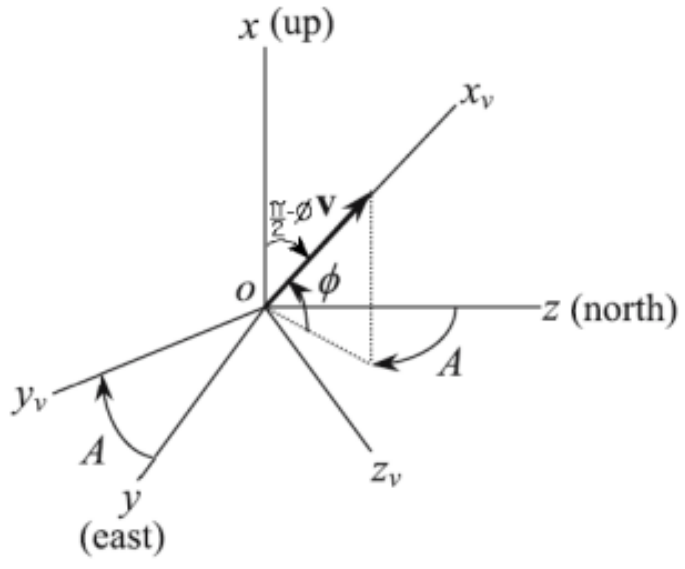
\includegraphics[width=1.5in]{figuras/vento.png}
        \label{fig:refvento}
        \fonte{\cite{livro:andre}}
     \end{center}
\end{figure}

A matriz de transformação do sistema LVLH para o SRV é definida pelo produto de matriz de rotação elementares:

\begin{equation}
C_{srv}^{lvlh} = 
 \left[\begin{array}{lll}
sin \phi & cos\phi sin A & cos\phi cos A \\
0 & cos A & -sinA \\
-cos \phi & sin \phi sin A & sin \phi cosA  
\end{array}\right]
\end{equation}

\subsection{Sistema referencial propulsivo}

O sistema de referência propulsivo é usado para definir o apontamento da força propulsiva com respeito ao SRV. A transformação do SRV para o SRP é encontrada a partir de uma sequência de rotações elementares:

\begin{equation}
C_{srp}^{srv} = 
 \left[\begin{array}{lll}
cos \mu cos \epsilon & sin \mu & -cos \mu sin \epsilon \\
-sin \mu cos \epsilon & cos \mi & sin \mu sin \epsilon \\
sin \epsilon & 0 & cos \epsilon  
\end{array}\right]
\end{equation}

\begin{figure}[h]
    \begin{center}
        \caption{SRP com respeito ao LVLH}
        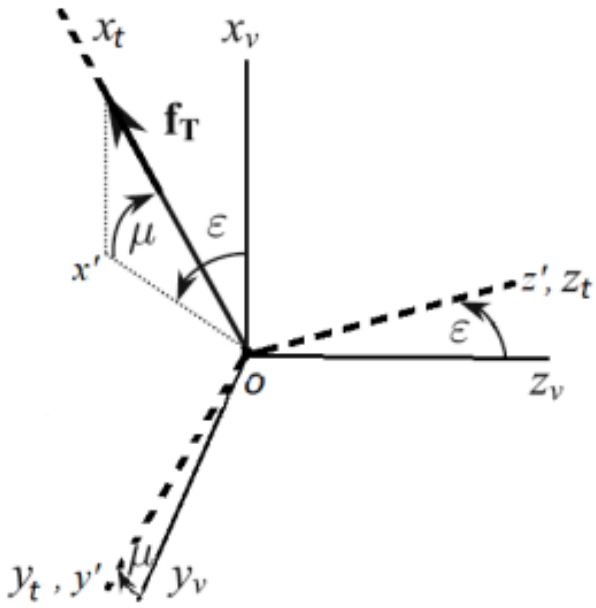
\includegraphics[width=1.5in]{figuras/srp.png}
        \label{fig:SRP}
        \fonte{\cite{livro:andre}}
     \end{center}
\end{figure}

 O SRP é mostrado na figura \ref{fig:SRP}, na qual a origem é o CM do veículo, o eixo $x_{t}$ aponta na direção da força propulsiva, o eixo $z_{t}$ está contido no plano $x_{v}z_{v}$ do SRV, e o eixo $y_{t}$ completa o sistema cartesiano ortogonal da mão direita. 

 \subsection{Força aerodinâmica}

 As forças aerodinâmicas escritas no SRV são dadas por:

 \begin{equation}
     f_{a_{srv}} = \left[\begin{array}{l}
-D \\
f_{y} \\
-L
\end{array}\right]
 \end{equation}

 A força de arrasto D têm sentido oposto à velocidade relativa, enquanto a força de sustentação L é perpendicular à força de arrasto, por fim, a força lateral é perpendicular ao vetor velocidade relativa. 

 \subsection{Força propulsiva}
 A força propulsiva que aponta ao longo do eixo $x_{t}$ com magnitude $f_{T}$ é escrita no SRP como:
\begin{equation}
     f_{T_{srp}} = \left[\begin{array}{l}
f_{T} \\
0 \\
0
\end{array}\right]
 \end{equation}

 No SRV, a força propulsiva é dada por:
\begin{equation}
     f_{T_{srv}} = \left[\begin{array}{l}
f_{T} cos \epsilon cos\mu\\
f_{T} sin\mu\\
-f_{T} cos \mu sin\epsilon
\end{array}\right]
 \end{equation}

Na qual os ângulos  $\mu$ e  $\epsilon$ são a angulação da tubeira em relação à velocidade relativa do veículo, que na prática são os ângulos do guimbal de 2 GDL responsáveis pela fatoração da tração. 

\subsection{Força gravitacional}

A força gravitacional é representada no referencial LVLH como:

\begin{equation}
     f_{g_{lvlh}} = m \left[\begin{array}{l}
-g_{c}\\
0\\
g_{\delta}
\end{array}\right]
 \end{equation}

Assim, a força gravitacional escrita no SRV é dada por:
\begin{equation}
     f_{g_{srv}} = m \left[\begin{array}{l}
-mg_{c}sin\phi + mg_{\delta}cos\phi cos A   \\
-mg\Delta sin A\\
mg_{c}cos\phi + mg_{\delta}sin\phi cos A  
\end{array}\right]
 \end{equation}

 \section{Dinâmica de translação}

 O modelo de mecânica de voo de translação do veículo possui seis equações diferenciais não lineares e três graus de liberdade, para os quais as variáveis de estado são as coordenadas esféricas da posição no referencial PCPF (distância radial $r$, longitude planetária $l$ e latitude $\delta$) e as coordenadas da velocidade relativa escritas no referencial LVLH (magnitude $v$, azimute da velocidade $A$ e elevação $\phi$). As equações são dadas por:


    
\begin{align}
\begin{split}
\dot{v} &= \frac{1}{m} (-D+f_{T}\cos \epsilon \cos\mu + mg_{c} \sin \phi + mg_{\delta} \cos A \cos \phi)\\
&\quad -r\omega_{e}^{2} \cos \delta (\cos A \sin \delta \cos \phi - \cos\delta \sin \phi)
\end{split}\\[1cm]
\begin{split}
\dot{A} &=  \frac{1}{mvcos\phi} (f_{y}+f_{T}\sin \mu - mg_{\delta} \sinA) - \frac{1}{vcos\phi} 2v\omega_{e} (\cosA\cos\delta \sin\phi - \sin\delta \cos\phi)\\
&\quad + \frac{1}{cosv\phi} (r\omega_{e}^{2} \sin A \sin \delta \cos \delta + \frac{v^{2}}{r} \sin A \tan\delta \cos^{2}\phi)
\end{split}\\[1cm]
\begin{split}
\dot{\phi} &= \frac{1}{mv}(L+f_{T} \cos \mu \sin\epsilon - mg_{c} \cos\phi - mg_{\delta}\cos A \sin \phi )\\
&\quad + \frac{1}{v}(2v\omega_{e} \sin A \cos\delta + \frac{v^{2}}{r} \cos \phi + r\omega_{e}^{2} \cos \delta (\cosA\sin\delta \sin\phi + \cos\delta \cos \phi))
\end{split}
\end{align}

%%%%%%%%%%%%% AULA 21 FIM 












































































%% Modelo Atmosferico aula 22

\section{Modelo Atmosférico}

Nesse contexto, vamos explorar os princípios de equilíbrio hidrostático e gás ideal para elaborar perfis verticais correspondentes à pressão, densidade e temperatura sob um estado estacionário de atmosfera padrão. Além disso, iremos estruturar uma variedade de parâmetros adimensionais essenciais para calcular as cargas aerodinâmicas e térmicas.

Ao descrever a atmosfera padrão, estabelecemos uma série de camadas sequenciais, que são caracterizadas pela variação do perfil de temperatura. Na Terra, as camadas são tradicionalmente designadas, em ordem crescente de altitude, como troposfera, estratosfera, mesosfera, termosfera e exosfera.

Algumas constantes termodinâmicas básicas são necessárias para configurar as camadas em equilíbrio termodinâmico. A equação que define a alteração linear da temperatura com a altitude em uma camada específica é:

\begin{equation}
T=T_{i}+a\left(h-h_{i}\right)
\end{equation}

Nessa equação, $i$ representa a camada em questão, $h$ é a altura geométrica e $a$ corresponde à taxa de lapso termal.

A taxa de lapso termal tem uma relação direta com o expoente politrópico $n$, que é crucial para avaliar a estabilidade do equilíbrio hidrostático em uma camada atmosférica. Conforme a seguinte equação, uma camada atmosférica é considerada termicamente estável se $a<0$ e instável se $a>0$.

\begin{equation}
a=-g \frac{1}{R} \frac{n-1}{n}
\end{equation}

Para valores de $a \neq 0$, a pressão como função da altitude geométrica nas camadas com variação linear de temperatura é definida como:

\begin{equation}
p=p_{i}\left(1+\frac{a\left(h-h_{i}\right)}{T_{i}}\right)^{-\frac{g_{0}}{R a}\left(1+\beta\left(\frac{T_{i}}{a}-h_{i}\right)\right)} \exp \left(\frac{g_{0} \beta}{R a}\left(h-h_{i}\right)\right)
\end{equation}

Nessa equação, $g_{0}$ denota a gravidade ao nível do mar, $R$ é a constante específica do gás e $\beta$ é definido por $\beta=2 / r_{0}$, onde $r_{0}$ é o raio médio da Terra.

No caso de camadas isotérmicas $(a=0)$, a pressão como função da altitude geométrica é expressa por:

\begin{equation}
p=p_{i} \exp \left(-\frac{g_{0}}{R T_{i}}\left(h-h_{i}\right)\left(1-\frac{\beta}{2}\left(h+h_{i}\right)\right)\right)
\end{equation}

Depois de calcular a temperatura e a pressão, podemos determinar a densidade utilizando a equação do gás ideal:

\begin{equation}
\rho=\frac{p}{R T}
\end{equation}

As expressões apresentadas são utilizadas para calcular a temperatura, a pressão e a densidade em qualquer altitude até $86 \mathrm{~km}$, faixa na qual a suposição de equilíbrio hidrostático ainda é válida.

Existem múltiplos padrões atmosféricos reconhecidos, com a taxa de variação da temperatura sendo um dos principais parâmetros usados como referência. No curso abordado, optou-se por um modelo misto, conforme proposto por Tewari (2007), que combina dois modelos distintos:

\begin{itemize}
\item No intervalo de $0 \leq h \leq 86 \mathrm{~km}$, aplica-se o padrão da atmosfera dos Estados Unidos de 1976. Este padrão contém duas camadas acima de $86 \mathrm{~km}$, que apresentam variação de temperatura não linear com a altitude e um certo grau de incerteza;

\item Para altitudes superiores a $86 \mathrm{~km}$, é usado o padrão atmosférico americano de 1962. Este padrão representa camadas até a altitude de $h=2000 \mathrm{~km}$, todas com temperatura variável linearmente. A combinação dos padrões atmosféricos dos Estados Unidos de 1976 e 1962 resulta em um modelo de 21 camadas (contando com as subcamadas). Esta combinação é ilustrada na figura abaixo.
\end{itemize}

\begin{figure}[h]
    \begin{center}
        \caption{Combinação de atmosfera padrão norte americana de 1976 e 1962}
        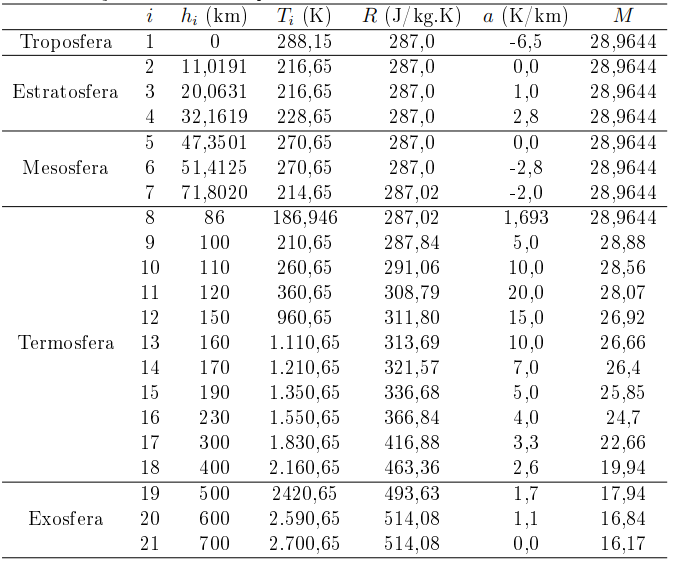
\includegraphics[width=3.5in]{figuras/atmos.png}
        \label{fig:atmos}
        \fonte{(TEWARI,2007), adaptado.}
     \end{center}
\end{figure}

Além das variáveis termodinâmicas básicas, alguns parâmetros adicionais podem ser calculados a partir do modelo atmosférico. Tais parâmetros são úteis para determinar cargas aerotérmicas:

\begin{enumerate}[(a)] 
\item Velocidade do som: 
\begin{equation}
a_{\infty}=\sqrt{\gamma R T}
\end{equation}
\end{enumerate}


\begin{enumerate}[(b)] 
\item Número de Mach:
\begin{equation}
M=\frac{v}{a_{\infty}}
\end{equation}
Onde $v$ representa a velocidade do veículo em relação à atmosfera.
\end{enumerate}

\begin{enumerate}[(c)] 
\item Coeficiente de viscosidade dinâmica:
\begin{equation}
\mu=1,458 \times 10^{-6} \frac{T^{\frac{3}{2}}}{T+110,4}
\end{equation}
\end{enumerate}

\begin{enumerate}[(d)] 
\item Número de Prandtl:
\begin{equation}
\operatorname{Pr}=\frac{\mu c_{p}}{k_{T}}
\end{equation}
Onde $k_{T}$ é o coeficiente de condutividade térmica do gás ideal, enquanto $c_{p}$ é seu calor específico a pressão constante, que pode ser calculado por:
\begin{equation}
c_{p}=\frac{R \gamma}{\gamma-1}
\end{equation}
\end{enumerate}

\begin{enumerate}[(e)] 
\item Número de Knudsen:
\begin{equation}
K n=\frac{\lambda}{l_{c}}
\end{equation}
Onde $\lambda$ é o caminho livre médio do fluxo não perturbado de moléculas e $l_{c}$ é um comprimento característico. O caminho livre médio é baseado no diâmetro de colisão $\sigma$, que pode ser calculado por:
\begin{equation}
\lambda=\frac{m}{\sqrt{2} \pi \sigma^{2} \rho N_{a}}
\end{equation}
Onde $m$ é a massa molecular em $\mathrm{kg} / \mathrm{Mol}$, e $N_{a}=6,0220978 \times 10^{23}$ é o número de Avogadro.
\end{enumerate}

\begin{enumerate}[(f)] 
  \item O parâmetro de regime de escoamento $d$, baseado no número de Knudsen:

  - Se $d=1$, o escoamento é livre molecular. Para $K n \geq 10$;

  - Se $d=2$, o escoamento é contínuo. Para $K n \leq 0,01$;

  - Quando $d=3$, o escoamento é de transição entre os dois regimes. Para $0,01<$ $K n<10$.
\end{enumerate}

\begin{enumerate}[(g)] 
\item Número de Reynolds:
\begin{equation}
R_e =\frac{\rho v l_{c}}{\mu}
\end{equation}
\end{enumerate}


\section{Modelo Gravitacional}

O modelo gravitacional utilizado é o mesmo utilizado no Trabalho 1, as principais hipóteses e pontos que devem ser reforçados são que um campo gravitacional conservativo, aplicado à segunda Lei de Newton para um corpo contínuo, permite a definição do potencial gravitacional:

\begin{equation}
g_i = \frac{\partial \phi_i}{\partial \mathbf{r}_{\mathbf{mi}}} = -Gm_i \frac{\mathbf{r}_{\mathbf{mi}}}{\left\|\mathbf{r}_{\mathbf{mi}}\right\|^3}
\end{equation}


Um modelo gravitacional para um corpo de simetria axial foi utilizado, levando em consideração o potencial gravitacional já descrito no Trabalho 1:

\begin{equation}
\Phi(r, \phi) = \frac{GM}{r}\left(1 - \sum_{n=2}^{\infty}\left(\frac{R_e}{r}\right)^n J_n P_n(\cos \phi)\right)
\end{equation}

Os polinômios de Legendre necessários para o cálculo do potencial são:

\begin{align}
P_2(v) &= \frac{1}{2}\left(3v^2 - 1\right) \\
P_3(v) &= \frac{1}{2}\left(5v^3 - 3v\right) \\
P_4(v) &= \frac{1}{8}\left(35v^4 - 30v^2 + 3\right)
\end{align}

Aplicando o gradiente à função potencial, é possível obter a aceleração da gravidade para coordenadas esféricas:

\begin{equation}
\frac{\partial \Phi}{\partial \mathbf{r}} = \frac{\partial \Phi}{\partial r} \mathbf{i}_r + \frac{\partial \Phi}{\partial \phi} \mathbf{i}_\phi + \frac{1}{r\sin \phi}\frac{\partial \Phi}{\partial \theta} \mathbf{i}_\theta
\end{equation}

\section{Modelo Aerodinâmico}

O modelo aerodinâmico desenvolvido abrange uma ampla faixa de regimes de escoamento, desde subsônico até hipersônico, levando em consideração a densidade do ar desde o meio contínuo até o livre molecular. Além disso, o modelo também incorpora diversos regimes de turbulência, bem como a dependência com a temperatura e reações químicas na termosfera e exosfera.

Em relação aos coeficientes de momento e força, geralmente são calculados três coeficientes de momento: rolagem ($C_{l}$), arfagem ($C_{m}$) e guinada ($C_{n}$); e três coeficientes de força: arrasto ($C_{D}$), sustentação ($C_{L}$) e lateral ($C_{Y}$). No entanto, neste contexto específico, apenas o movimento de translação do foguete é considerado, portanto, os coeficientes de momento não serão modelados. Os coeficientes de força serão avaliados de acordo com as seguintes hipóteses:

\begin{itemize}
    \item Foguetes são otimizados para baixa razão estrutural, o que implica que eles suportam baixos fatores de carga normais ou laterais. Portanto, voam com baixo ângulo de ataque e derrapagem, resultando em forças de sustentação e lateral muito pequenas, as quais podem ser consideradas nulas no modelo.
\end{itemize}

Dentro dessas limitações, apenas o coeficiente de arrasto será tratado. No voo de foguetes, o arrasto é importante para avaliar a perda de velocidade $\Delta v$ que o veículo sofre devido à resistência atmosférica.

Devido à complexidade em estimar modelos de arrasto, será adotado o modelo apresentado na referência (TEWARI, 2007), que é aplicável a uma cápsula de reentrada. No entanto, outros modelos também serão revisados a fim de fazer adaptações no modelo de referência.

Assumiremos que o veículo possui estabilidade estática, o que implica que os ângulos de ataque e derrapagem permaneçam nulos. Nesse caso, o coeficiente de arrasto da cápsula, para uma área de referência da base da cápsula de $S=4 \mathrm{~m}^{2}$, é dado por:

\begin{equation}
\left\{
\begin{array}{lr}
C_{D}=C_{D_{c}} & \text{se } K n<0,0146 \\
C_{D}=C_{D_{f m}} & \text{se } K n>14,5 \\
C_{D}=C_{D_{c}}+\left(C_{D_{f m}}-C_{D_{c}}\right)\left(\frac{1}{3} \log _{10} \frac{K n}{\sin 30^{\circ}}+0,5113\right) & \text{se } 0,0146 \leq K n \leq 14,5
\end{array}
\right.
\end{equation}

onde $K n$ é o número de Knudsen, calculado para o comprimento de referência $l_{c}=0,5 \mathrm{~m}$; $C_{D_{c}}$ é o coeficiente de arrasto no meio contínuo; e $C_{D_{f m}}$ é o coeficiente de arrasto no regime de escoamento livre molecular. O coeficiente $C_{D_{c}}$ é plotado como uma função do número de Mach, conforme ilustrado na Figura \ref{fig:aerodin}.

\begin{figure}[H]
    \begin{center}
        \caption{Coeficiente de arrasto contínuo em função do número de Mach}
        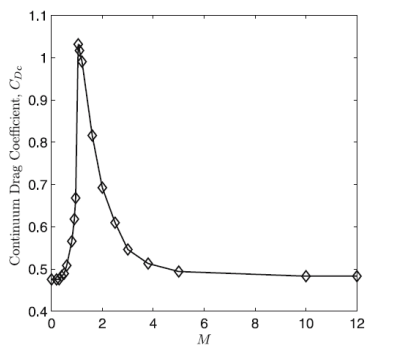
\includegraphics[width=3.5in]{figuras/mach.png}
        \label{fig:aerodin}
        \fonte{(TEWARI,2007).}
     \end{center}
\end{figure}

Podemos ver a partir da Figura \ref{fig:aerodin}, que o princípio de independência do número de Mach hipersônico é válido, tendo em vista que $C_{D_c}$ torna-se invariante com o número de Mach para $M > 8$.




\section{Voo ascendente de foguete}

A partir dos modelos desenvolvidos anteriormente, é possível simular o voo ascendente de um foguete, que possui duas aplicações de interesse: voo de sondagem e voo de inserção orbital.

No voo de sondagem, a trajetória é vertical ou quase vertical, com o objetivo principal de varrer uma faixa de altitude. Geralmente, a missão tem como objetivo adquirir dados em função da altitude ou realizar experimentos em microgravidade. Nesse tipo de trajetória, é necessário que o foguete mantenha uma trajetória vertical de forma estável, geralmente de maneira balística, sem a execução de manobras. Quando o veículo atinge a altitude máxima que atende aos objetivos da missão, a velocidade relativa se aproxima de zero ou se torna muito pequena.

Quanto ao voo de inserção orbital, também é lançado verticalmente ou próximo disso. No entanto, durante a ascensão, a trajetória deve curvar-se gradualmente, de modo que, no momento em que o motor do último estágio é desligado, o ângulo da trajetória seja próximo ou igual a zero. Ao atingir a altitude orbital e desligar o motor do último estágio, a velocidade relativa não será nula. Nesse momento, a velocidade do veículo deve ser igual à velocidade orbital desejada. Portanto, não basta apenas atingir a altitude desejada, mas também é necessário fornecer um impulso de velocidade compatível com a órbita naquela altitude.

A trajetória de inserção orbital pode envolver manobras ou ocorrer de forma puramente balística, dependendo do nível de precisão desejado, das características dos motores, da estabilidade e do controle. Independentemente da presença ou ausência de manobras, a trajetória deve garantir que o ângulo de trajetória seja próximo ou igual a zero no momento da inserção orbital, quando os motores são desligados.

Além das equações de movimento, do modelo aerodinâmico genérico, do modelo atmosférico e do modelo gravitacional mencionados anteriormente, é necessário especificar algumas características básicas do veículo:

\begin{itemize}
    \item Número de estágios;
    \item Massa de propelente de cada estágio;
    \item Massa estrutural de cada estágio;
    \item Massa da carga útil;
    \item Modelo propulsivo de cada estágio: tração e consumo de propelente;
    \item Parâmetros aerodinâmicos de cada estágio.
\end{itemize}

Se o foguete é de múltiplos estágios (N estágios), é necessário inserir na modelagem uma lógica de sequenciamento, a qual deve conter:

\begin{itemize}
    \item Tempo de ignição $t_{i_{k}}$ do estágio $k$, para $k = 1, \ldots, N$. Isso representa o momento em que o k-ésimo estágio é ligado.
   \item Tempo de queima $t_{q_{k}}$ do estágio $k$, para $k = 1, \ldots, N$. Isso representa o momento em que o k-ésimo estágio é desligado.
   \item Tempo de separação $t_{s_{k}}$ do estágio $k$, para $k = 1, \ldots, N$. Isso representa o momento em que o k-ésimo estágio é separado.
\end{itemize}

O sequenciamento de tempos da missão pode ser escrito de maneira relativa:

\begin{itemize}
    \item $t_{i_{k}} = t_{s_{k-1}} + T_{i_{k}}$, para $k = 2, \ldots, N$, onde $T_{i_{k}}$ é o tempo de espera para a ignição do estágio $k$ após a separação do estágio $k-1$.
    \item $t_{q_{k}} = t_{i_{k}} + T_{q_{k}}$, para $k = 1, \ldots, N$, onde $T_{q_{k}}$ é o tempo de duração da queima de propelente do motor do estágio $k$.
    \item $t_{s_{k}} = t_{q_{k}} + T_{s_{k}}$, para $k = 1, \ldots, N$, onde $T_{s_{k}}$ é o tempo de espera para a separação do estágio $k$ após a queima de seu propelente.

\end{itemize}


\subsection{Modelo Propulsivo}

Para o modelo propulsivo é necessário desenvolver os modelos de tração e variação de massa. Para um foguete com $N$ estágios, a variação de massa depende do desacoplamento dos estágios e do consumo de propelente pelos motores. Para os cálculos assumimos uma curva conhecida para a tração em função do tempo. Para determinar a massa em função do tempo, a partir da curva de tração fornecida, podemos utilizar a definição de impulso específico e a fórmula da tração reativa:

\begin{equation}
v_{e_{k}} = g I_{sp_{k}}, \quad f_{T_{k}}(t) = \dot{m}_{p_{k}} v_{e_{k}}
\end{equation}

Assumimos que a variação da tração devido à pressão no bocal de exaustão esteja modelada no impulso específico $I_{sp_{k}}$ ou na velocidade de exaustão $v_{e_{k}}$. Portanto, podemos determinar a relação entre $f_{T_{k}}(t)$ e $\dot{m}_{p_{k}}$ da seguinte forma:

\begin{equation}
\dot{m}_{p_{k}} = \frac{f_{T_{k}}(t)}{g I_{sp_{k}}}
\end{equation}

A vazão mássica de propelente $\dot{m}_{p_{k}}$ e a variação de massa do veículo $\dot{m}$ possuem sinais opostos, pois a vazão de propelente implica na diminuição da massa do veículo. Portanto, para calcular a taxa de variação da massa do veículo, trocamos o sinal de $\dot{m}_{p_{k}}$:

\begin{equation}
\dot{m} = -\frac{f_{T_{k}}(t)}{g I_{sp_{k}}}
\label{eq:252}
\end{equation}

Conhecendo a curva de tração em cada estágio durante a queima de propelente e a lógica de sequenciamento de estágios, o modelo da força propulsiva em função do tempo é dado por:

\begin{equation}
f_{T}(t) = 
\begin{cases}
f_{T_{k}}(t) & , \quad t_{i_{k}} \leq t \leq t_{q_{k}} \\
0 & , \quad t_{q_{k}} < t < t_{i_{k+1}}
\end{cases}
\end{equation}

Como o estágio $k+1$ não inicia sua queima instantaneamente após o estágio $k$, há um intervalo de tempo $\left(t_{q_{k}}, t_{i_{k+1}}\right)$ no qual nenhuma tração é aplicada. Esse intervalo tem duração $T_{s_{k}}+T_{i_{k+1}}$ e é chamado de fase de voo balístico. Em veículos lançadores de propulsão sólida e sem vetorização de tração, as únicas variáveis de controle são os tempos de duração das fases de voo balístico, ou seja, os intervalos de tempo $\left(t_{q_{k}}, t_{i_{k+1}}\right)$.

A lógica para determinação da massa, estágio após estágio, pode ser vista na equação condicional abaixo:

\begin{equation}
m(t) = 
\begin{cases}
m_{0_{1}} = m_{0} & , \quad t_{0} \leq t < t_{i_{1}} \\
m_{0_{k}} - \Delta m_{p_{k}}(t) & , \quad t_{i_{k}} \leq t \leq t_{q_{k}} \\
m_{0_{k}} - m_{p_{k}} & , \quad t_{q_{k}} < t < t_{s_{k}} \\
m_{0_{k+1}} = m_{0_{k}} - m_{p_{k}} - m_{s_{k}} & , \quad t_{s_{k}} \leq t < t_{i_{k+1}}
\label{eq:516}
\end{cases}
\end{equation}



A variável $\Delta m_{p_{k}}(t)$ na Equação \ref{eq:516} é definida como:

\begin{equation}
\Delta m_{p_{k}}(t) = \int_{t_{i_{k}}}^{t} \frac{f_{T_{k}}(\tau)}{g I_{sp_{k}}} d \tau
\end{equation}

No qual assumimos que:

\par - Toda a massa de propelente é consumida durante a queima de cada estágio;
\par - O desacoplamento de cada estágio é instantâneo.

\section{Algoritmos}

Todos os algoritmos desenvolvidos foram feitos de acordo com o fornecido pelo professor e adaptados de acordo com a necessidade do grupo. Os passos gerais do programa são:

\begin{itemize}
    
    \item Dados do veículo lançador e carga paga;

    \item Parâmetros de queima dos estágios;

    \item Parâmetros gerais do lançamento;

    \item Função que cálculo a dinâmica do movimento do veículo lançador;

    \item Funções auxiliares para os cálculos da dinâmica;

    \item Determinação dos parâmetros gerais da órbita;

    \item Plotagem dos gráficos.
    
\end{itemize}

Os programas elaborados para as aulas 19, 26 e 27 foram estruturados com uma função principal em um arquivo, complementada por diversas funções auxiliares dispostas em arquivos separados. No entanto, durante a criação dos códigos para a aula 29, que originalmente seguiam a mesma estrutura, enfrentamos inúmeros problemas relacionados à importação e declaração de variáveis globais, bem como aos inputs de funções.

Isso nos levou a adotar a estratégia de compilar todo o código em um único arquivo. Embora essa alteração tenha aumentado a demanda de processamento para a execução do código, ela permitiu solucionar os erros encontrados e efetivar a transposição do código do Matlab para Python.

É importante enfatizar que essa decisão foi tomada considerando o volume de erros encontrados e o prazo limitado que tínhamos à disposição. Apesar da demanda computacional adicional, consideramos essa medida necessária para cumprir o cronograma estabelecido.
\chapter{Resultados}

A equação do foguete, juntamente com os modelos e conceitos discutidos anteriormente, pode ser aplicada de forma prática para estudar diferentes configurações de veículos lançadores e suas capacidades de inserção de carga útil em órbita geossíncrona.

Com base nas aulas ministradas, é utilizado o veículo lançador brasileiro VLM-1 como ponto de partida, no qual podemos propor novos arranjos capazes de realizar diferentes missões de lançamento. O veículo lançador utiliza os motores S-44 e S-50, com seus dados de massa, de impulso específico e tração média. Esses dados são apresentados na Tabela \ref{tab:daods}.


\begin{table}[H]
\centering
\caption{Dados dos motores S-50 e S-44.} % Título da tabela
\label{tab:daods}
\begin{tabular}{@{}lllll@{}}
\toprule
Motor & $m_{p}[\mathrm{~kg}]$ & $m_{s}[\mathrm{~kg}]$ & $I_{s p}[\mathrm{~s}]$ & $\bar{F}[\mathrm{kN}]$ \\ \midrule
S-50  & 11058                 & 1367                  & 271                    & 440                    \\ 
S-44  & 813                   & 166,5                 & 270                    & 38                     \\ \bottomrule
\end{tabular}
\fonte{Notas de aula.} % Nota de rodapé
\end{table}

Também foi utilizado o motor RD-843, suas especificações podem ser vistas na Tabela \ref{tab:rdd}.

\begin{table}[H]
\centering
\caption{Dados do motor RD-843.} % Título da tabela
\label{tab:rdd}
\begin{tabular}{@{}ccccc@{}}
\toprule
Massa               & Tração             & Impulso específico & Número de queimas & Tempo de operação \\ \midrule
16,5 kg             & 2,5 kN             & 315,5 s            & 5                  & 700 s             \\ \bottomrule
\end{tabular}
\fonte{Notas de aula.} % Nota de rodapé
\end{table}

As configurações propostas são modificadas, alterando valores de parâmetros que serão exemplificados mais posteriormente.


Essa aplicação prática permitirá explorar e analisar diferentes configurações de veículos lançadores, considerando as restrições e requisitos específicos para alcançar uma órbita geossíncrona, e avaliar a viabilidade e desempenho desses sistemas para a realização da missão proposta.


%\begin{figure}[H]
%    \begin{center}
%        \caption{Coeficiente de arrasto contínuo em função do número de Mach}
%        \includegraphics[width=3.5in]{figuras/.png}
%        \label{fig:aerodin}
%       \fonte{(TEWARI,2007).}
%     \end{center}
%\end{figure}

\section{Impulso de Velocidade}

A primeira avaliação para a inserção orbital de um veículo lançador é realizada por meio do cálculo da capacidade de impulso de velocidade, $\Delta v$. Essa avaliação consiste em determinar a capacidade de $\Delta v$ de uma determinada configuração de veículo lançador para uma carga útil específica, conforme apresentado na seção \ref{sectionfoguete}.

No contexto da inserção em órbita geossíncrona, o requisito de $\Delta v$ necessário foi mencionado pelo professor durante a aula como $\Delta v_{req} = 13 km/s$. Esse valor representa o impulso total necessário para atingir a órbita geossíncrona, levando em consideração as perdas esperadas durante o lançamento, como a perda de arrasto.

Durante a avaliação, o valor de $\Delta v_{req}$ da configuração do veículo lançador é comparado com valores tabelados aproximados, levando em conta as perdas esperadas, a fim de determinar se a configuração proposta é capaz de atender ao requisito de $\Delta v_{req}$ para a inserção orbital geossíncrona.

Essa avaliação é crucial para garantir que o veículo lançador tenha a capacidade necessária para inserir a carga útil na órbita desejada e alcançar os objetivos da missão proposta.

Para a resolução desse parâmetro foi utilizado o código \textit{"estudo\_equacao\_foguete"}. O código é dividido em várias seções, começando com a definição de constantes, seguida dos dados das massas estruturais, massas de propelente e impulso específico ideal para cada configuração de foguete.

Em seguida, são realizados os cálculos, incluindo a determinação das razões estruturais, das massas totais no início da queima de cada estágio e das razões de carga útil para cada estágio e para a carga útil total. Esses cálculos são feitos para cada configuração de foguete.

A primeira simulação foi realizada com o três configurações apresentadas pelo professor em aula, C1, C2 e C3. OS dados de cada configuração podem ser vistos em \ref{tab:primeira}. Os dados já são apresentados considerando o acoplamento dos motores, considerando 550 kg de elementos de fixação no primeiro estágio e pequenas reduções no desempenho dos motores devido
às perturbações dos motores acoplados.

\begin{table}[H]
\centering
\caption{Dados das configurações de foguetes.}
\label{tab:primeira}
\begin{tabular}{ccccccc}
\toprule
Configuração & Estágio & Motores & $m_{p}[\mathrm{kg}]$ & $m_{s}[\mathrm{kg}]$ & $I_{s p}[\mathrm{s}]$ & $F[\mathrm{kN}]$ \\
\midrule
C-1 & 1 & $3 \times S-50$ & 33157 & 4650 & 251 & 1317 \\
 & 2 & $1 \times S-50$ & 11058 & 1367 & 271 & 455 \\
 & 3 & $1 \times S-44$ & 813 & 166,5 & 270 & 33 \\
\midrule
C-2 & 1 & $3 \times S-50$ & 33157 & 4650 & 251 & 1317 \\
 & 2 & $1 \times S-50$ & 11058 & 1367 & 271 & 455 \\
 & 3 & $1 \times R D-843$ & 609 & 161,9 & 315 & 2,5 \\
\midrule
C-3 & 1 & $3 \times S-50$ & 33157 & 4650 & 251 & 1317 \\
 & 2 & $1 \times S-50$ & 11058 & 1367 & 271 & 455 \\
 & 3 & $4 \times R D-843$ & 811 & 228,7 & 315 & 10 \\
\bottomrule
\end{tabular}

\fonte{Notas de aula.}
\end{table}

A partir do códigos, temos na Tabela \ref{tab:primeirosdados}, os resultados para essas configurações. Observa-se que para todos os casos o $\Delta v < \Delta v_{req}$, fazendo com que a escolha de configuração seja rejeitada.

\begin{table}[H]
\centering
\caption{Valores de $\Delta v$ para as configurações C-1, C-2 e C-3.}
\label{tab:primeirosdados}
\begin{tabular}{cccc}
\toprule
Configuração & C-1 & C-2 & C-3 \\
\midrule
$\Delta v[\mathrm{km} / \mathrm{s}]$ & 11,712 & 12,041 & 11,669 \\
\bottomrule
\end{tabular}

\fonte{Autores.}
\end{table}

Após isso foram feitas outras simulações, alterando os parâmetros da a configuração 2, a qual foi que a gerou resultados mais precisos na primeira simulação. Foi feito uma varredura utilizando o código \textit{"estudo\_foguete\_otimizado"}, no qual foram comparados os desempenhos de utilizar 3xS50, 4xS50, 5xS50 ou 7xS50 no primeiro estágio, e variando a massa de propelente do 3 estágio. 

Os resultados para essa simulação podem ser vistos na Figura \ref{fig:motores}, e nela é possível ver que a configuração de foguete com 7 motores S50 atinge a maior mudança de velocidade ($\Delta v$) quando a massa de propelente do terceiro estágio é aumentada em cerca de $37\%$. Nesse ponto, temos que $\Delta v = 13,34 km/s$, o que satisfaz o pré requisito.

\begin{figure}[H]
    \begin{center}
        \caption{Variação do $\Delta v$ para diferentes configurações}
        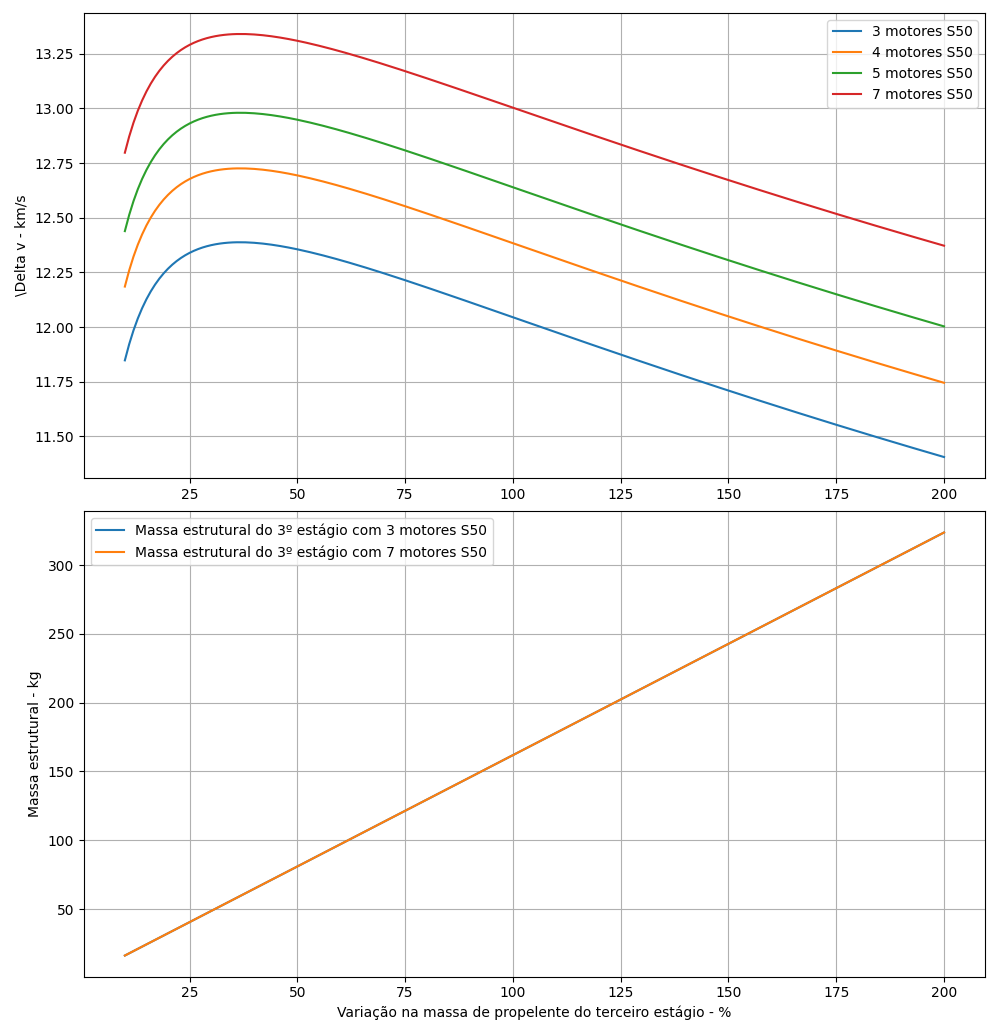
\includegraphics[width=4.5in]{figuras/motores.png}
        \label{fig:motores}
      \fonte{Autores.}
     \end{center}
\end{figure}

Portanto, a configuração final do foguete pode ser vista na Tabala \ref{tab:final}.

\begin{table}[h]
\centering
\caption{Configuração Final} 
\label{tab:final}
\begin{tabular}{cccccc}
\hline
Estágio & Motores & $m_{p}[\mathrm{~kg}]$ & $m_{s}[\mathrm{~kg}]$ & $I_{s p}[\mathrm{~s}]$ & $F[\mathrm{kN}]$ \\
\hline
1 & $7 \times S-50$ & 77366 & 7750 & 251 & 3073 \\
2 & $1 \times S-50$ & 11058 & 1367 & 271 & 455 \\
3 & $1 \times R D-843$ & 225.33 & 64.75 & 315 & 2.5 \\
\hline
\end{tabular}

\fonte {Autores.}
\end{table}

\section{Energia Específica}

A configuração, uma vez testada pela primeira vez, é submetida à análise de viabilidade com relação à energia específica. No contexto do caso em discussão, o objetivo é atingir uma órbita geossíncrona (GSO - Geosynchronous orbit), identificada por uma velocidade orbital de $n_{\text{gso}} = 7.2921 \times 10^{-5} \text{rad/s}$ e semieixo maior $a_{\text{gso}}= 42.164 \times 10^{6} \text{m}$ (6.61 vezes o raio da Terra).

Para a realização da verificação, escolhemos uma órbita circular de referência com raio $r_{\text{ref}} = a_{\text{gso}} = 42.164 \times 10^{6} \text{m}$, correspondente a uma altitude $h_{\text{ref}} = 35.785863 \times 10^{6} \text{m}$. Se a energia específica, no instante da inserção na órbita, exceder esse valor, tal órbita é alcançável por tal veículo, necessitando apenas de uma modificação das condições quando o motor do terceiro estágio for desligado.

A inspeção do voo de sondagem é realizada de maneira eficaz com base na velocidade relativa e na posição no referencial rotativo PCPF.Para isso foram utilizados os códigos que dizem respeito as dinâmicas do foguete, e os principais resultados podem ser vistos na Figura \ref{fig:sondagem}. 

Os dados utilizados para rodar o programa \textit{"voo\_sondagem\_3\_estagios"} foram os mesmo fornecidos como output do código \textit{"estudo\_foguete\_otimizado"}, sendo eles:

\begin{table}[h]
\centering
\caption{Dados para rodar o voo de sondagem} 
\label{tab:final}
\begin{tabular}{cccccc}
\hline
Estágio & Motores & $m_{p}[\mathrm{~kg}]$ & Tempo de queima [s]\\
\hline
1 & $S-50$ & 77366 &  62 \\
2 & $S-50$ & 11058 & 62 \\
3 & $R D-843$ & 225.33 & 278.43 \\
\hline
\end{tabular}

\fonte {Autores.}
\end{table}

\begin{figure}[H]
    \begin{center}
        \caption{Voo de sondagem.}
        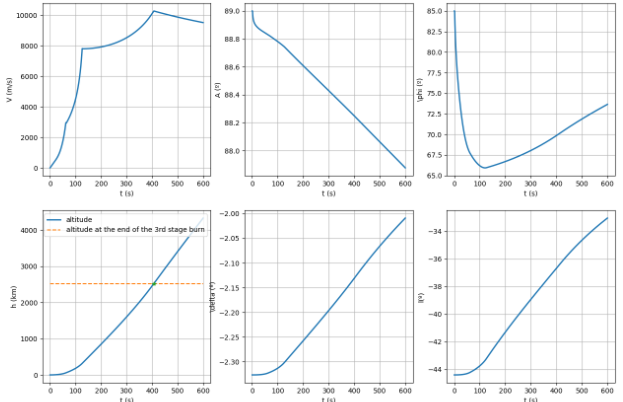
\includegraphics[width=6in]{figuras/voosondagema.png}
        \label{fig:sondagem}
      \fonte{Autores.}
     \end{center}
\end{figure}
\newpage


Porém, para estudar a inserção na órbita, é necessário calcular a velocidade inercial e a posição no referencial inercial ICP, a partir das quais os parâmetros orbitais podem ser avaliados. Então esses resultados são convertidos e podem ser vistos na Figura \ref{fig:parametrossondagem}.

\begin{figure}[H]
    \begin{center}
        \caption{Parâmetros inerciais do voo de sondagem.}
        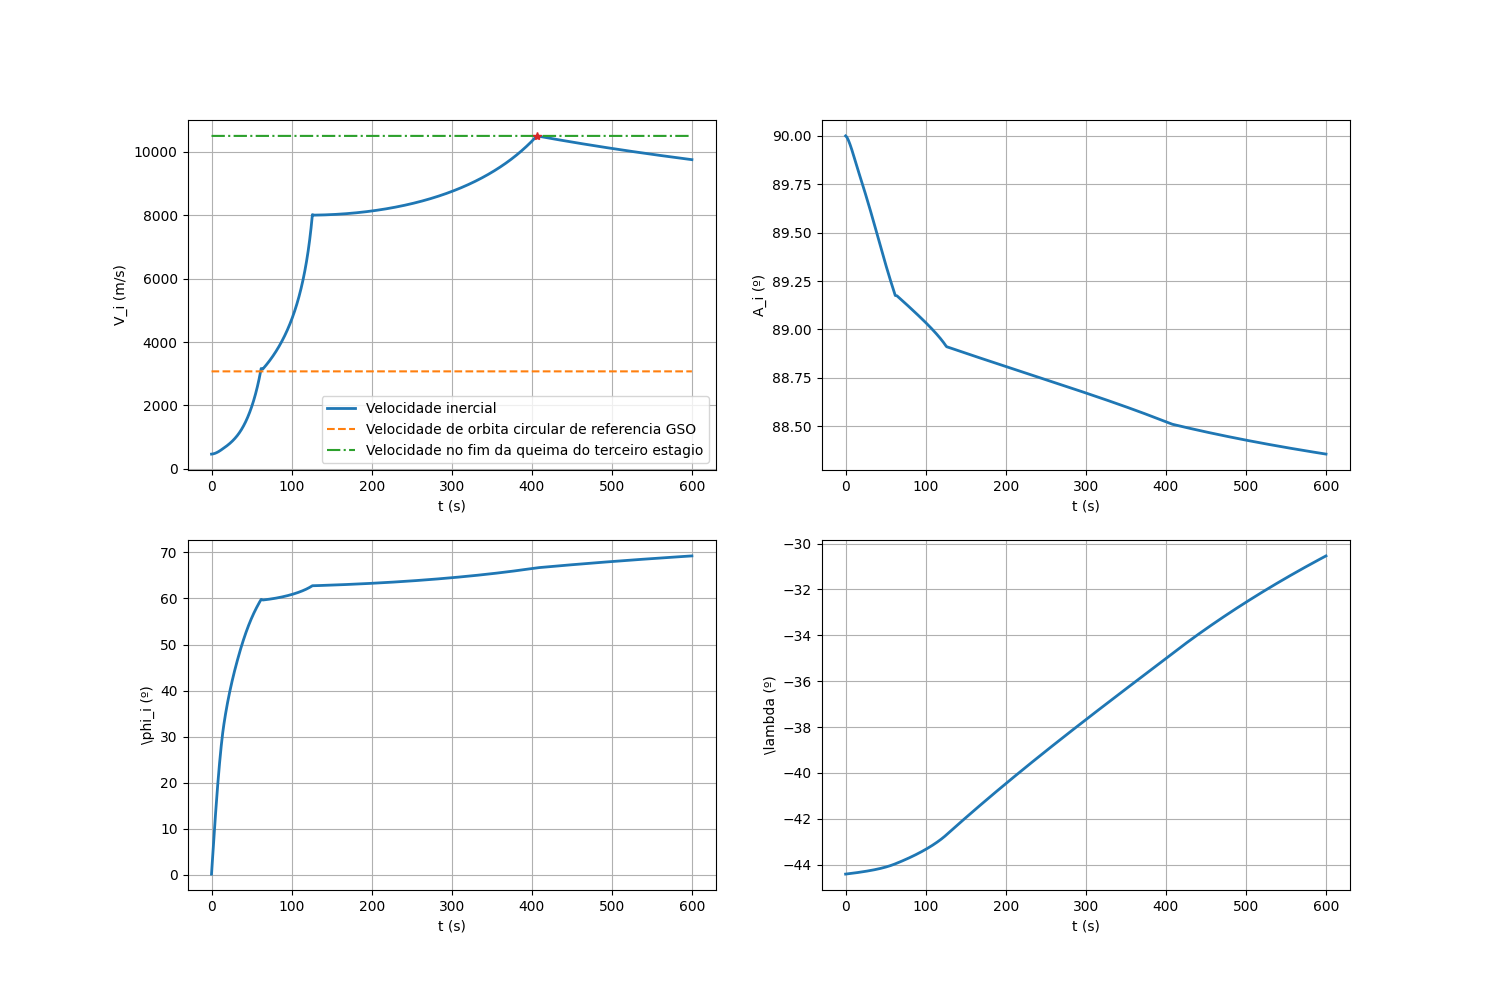
\includegraphics[width=7in]{figuras/parametrossondagem.png}
        \label{fig:parametrossondagem}
      \fonte{Autores.}
     \end{center}
\end{figure}

\newpage

Os parâmetros inerciais, incluindo a velocidade inercial e a posição no referencial inercial, são fundamentais para a determinação dos parâmetros orbitais. Ao utilizar código como o \textit{"det\_orbita"}, é possível computar estes parâmetros orbitais. Além disso, o código \textit{"calcula\_auxiliares"} é utilizado para calcular a energia específica do voo de sondagem. Os resultados podem ser vistos na Figura \ref{fig:energiaespecificasondagem}.


\begin{figure}[H]
    \begin{center}
        \caption{Energia específica e parâmetros orbitais.}
        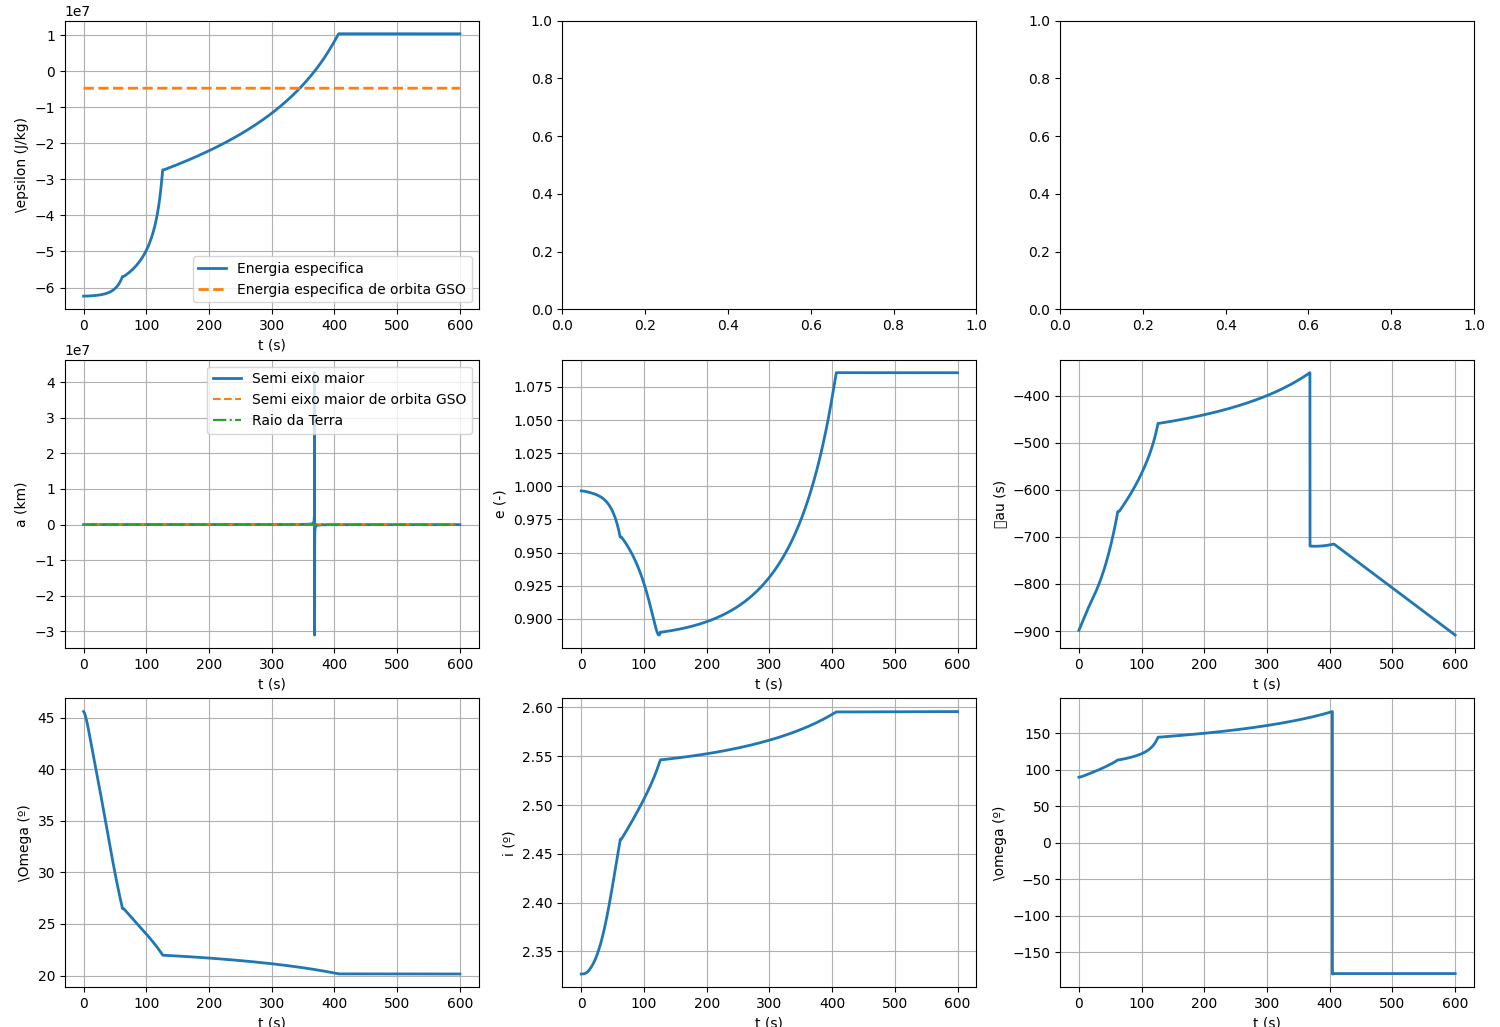
\includegraphics[width=5.8in]{figuras/energiaespecificasondagem.png}
        \label{fig:energiaespecificasondagem}
      \fonte{Autores.}
     \end{center}
\end{figure}

A interpretação mais importante dessa figura é a de no primeiro gráfico, a linha pontilhada representa a energia de referência necessária para atingir a órbita do problema, e a azul é a energia específica do foguete. Percebe-se que no momento que ocorre a inserção orbital, o foguete possui energia suficiente para tal.

Na Figura \ref{fig:3} podemos observar os tempos de queima de cada estágio, sendo os dois estágios iniciais com maior tempo de queima e maior empuxo gerado, enquanto o terceiro estágio possui uma única queima, rápida e com baixo empuxo gerado, que praticamente não pode ser observado sem zoom na imagem. Além disso, é possível notar a diminuição de massa após a massa ser ejetada durante a queima. 

\begin{figure}[H]
    \begin{center}
        \caption{Tempo de queima dos estágios.}
        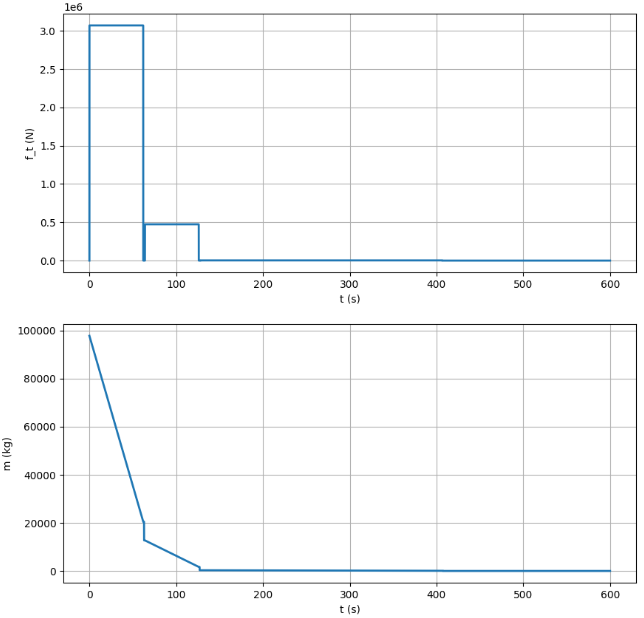
\includegraphics[width=3.4in]{figuras/fig3aula27.png}
        \label{fig:3}
      \fonte{Autores.}
     \end{center}
\end{figure}

Já na Figura \ref{fig:4} são plotados os resultados referentes as condições atmosféricas. Durante o lançamento, o arrasto, a densidade do ar e também a pressão dinâmica são maiores nos primeiros instantes, enquanto a temperatura tende a aumentar ao longo do lançamento. O número de Mach sofre grandes variações até aproximadamente três minutos após o lançamento, quando tende a se estabilizar.

\begin{figure}[H]
    \begin{center}
        \caption{Condições atmosféricas.}
        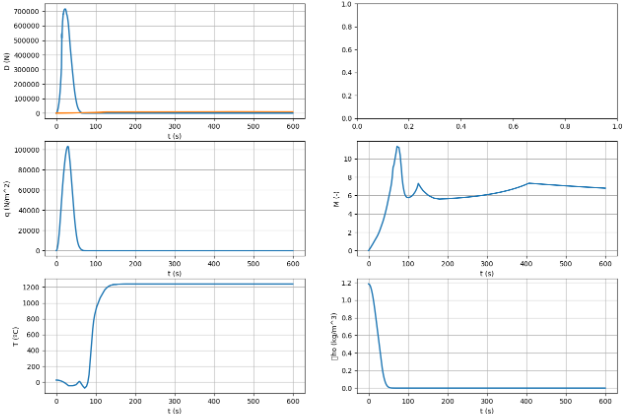
\includegraphics[width=4.5in]{figuras/fig4aula27a.png}
        \label{fig:4}
      \fonte{Autores.}
     \end{center}
\end{figure}

\section{Inserção em órbita GSO}
%%%%%%%% AULA 28%%%%%%%5
Para viabilizar a órbita GSO, é necessário utilizar do reacendimento do motor, que é a capacidade de um foguete ligar novamente, ou reacender, seus motores após eles terem sido desligados inicialmente. No caso do trabalho, isso é dado por múltiplas ignições do motor do último estágio, que é ignitado duas vezes. No caso, a primeira ignição coloca o foguete em órbita baixa com periastro numa altitude suficiente para sofrer baixo arrasto atmosférico, podendo essa ser uma órbita circular (estacionamento) ou excêntrica (transferência). Como a órbita utilizada é a de transferência, é necessário controlar o tempo de queima do último estágio em termos da elevação inercial da velocidade. Quando o ângulo de trajetória da velocidade inercial for zero, é necessário desligar o motor do último estágio, sendo esse o perigeu da órbita de transferência. Nesse momento, a velocidade inercial deve ser compatível com a velocidade de perigeu da órbita de transferência cujo apogeu é igual ao raio da órbita desejada, que é a órbita geossíncrona. 

Os dados de tempo de queima utilizados para a simulação foram:

\begin{table}[h]
\centering
\caption{Tempos de ignição e queima.}
\begin{tabular}{|c|c|}
\hline
\textbf{Descrição} & \textbf{Tempo (s)} \\
\hline
Tempo de Ignição & 580 \\
\hline
Tempo de Queima 1 & 213 \\
\hline
Tempo de Queima 2 & 66 \\
\hline
\end{tabular}

\fonte {Autores.}
\end{table}


Após adaptar os códigos e inserir os valores definidos, são gerados os outputs mostrados nas tabelas a seguir.

\begin{table}[H]
\centering
\caption{Parâmetros do foguete}
\begin{tabular}{|l|l|}
\hline
\textbf{Parâmetro} & \textbf{Valor} \\
\hline
Área ref. com 1o estágio ($m^2$) & 7.666666666666667 \\
Área ref. com 2o estágio ($m^2$) & 1.2345485272815064 \\
Área ref. com 3o estágio ($m^2$) & 0.977426364075326 \\
Área ref. da carga útil ($m^2$) & 0.786214389183969 \\
Massa ini. ant. queim. do 1o estágio (kg) & 97844.0844 \\
Massa ini. ant. queim. do 2o estágio (kg) & 12728.0844 \\
Massa ini. ant. queim. do 3o estágio (kg) & 303.0844 \\
Massa da carga útil (kg) & 13 \\
Razões estruturais & [0.09105221 0.11002012 0.22322607] \\
Razões de carga útil & [0.13008537 0.02381226 0.04289234] \\
Velocidades de exaustão (m/s) & [2461.46915 2657.60215 3089.09475] \\
Razão de carga útil total & 0.00013286444530314395 \\
Impulso de velocidade total ideal (m/s) & 13449.786837505853 \\
Cond. fin. de azimute de vel. inercial (grau) & 85.5731667395659 \\
Cond. ini. de azimute de vel. relativa (grau) & 85.35329334311488 \\
\hline
\end{tabular}

\fonte {Autores.}
\end{table}

\begin{table}[H]
\centering
\caption{Órbita GSO requerida}
\begin{tabular}{|l|l|}
\hline
\textbf{Parâmetro} & \textbf{Valor} \\
\hline
Raio da órbita GSO (km) & 42164.14 \\
Velocidade da órbita GSO (km/s) & 3.0746611796284924 \\
\hline
\end{tabular}

\fonte {Autores.}
\end{table}

\begin{table}[H]
\centering
\caption{Parâmetros da Órbita Obtida}
\begin{tabular}{|l|l|}
\hline
\textbf{Parâmetro} & \textbf{Valor} \\
\hline
Velocidade no momento da inserção orbital (km/s) & 7.915448092085045 \\
Altitude no momento da inserção orbital (km) & 3718.864788180722 \\
Distância radial no momento da inserção orbital (km) & 10097.001788180722 \\
Semi eixo maior (km) & 24454.165121965787 \\
Período (min) & 168.28615193314312 \\
Raio do perigeu (km) & 5474.673352743322 \\
Raio do apogeu (km) & 43433.65689118826 \\
Altitude do perigeu (km) & -903.463647256678 \\
Altitude do apogeu (km) & 37055.519891188254 \\
\hline
\end{tabular}

\fonte {Autores.}
\end{table}

\begin{table}[H]
\centering
\caption{Parâmetros da Órbita GTO Requerida}
\begin{tabular}{|l|l|}
\hline
\textbf{Parâmetro} & \textbf{Valor} \\
\hline
Perigeu da órbita GTO requerida (km) & 5474.673352743322 \\
Apogeu da órbita GTO requerida (km) & 42164.14 \\
Semi eixo maior da órbita GTO requerida (km) & 23819.406676371662 \\
Velocidade de perigeu da órbita GTO requerida (km/s) & 11.352615669084885 \\
Velocidade de apogeu da órbita GTO requerida (km/s) & 1.4740455393487284 \\
T disparo do propulsor do 3o estágio após a separação do 2º (s) & 580 \\
Duração do 1o disparo do motor do 3o estágio (s) & 215 \\
Duração do 2o disparo do motor do 3o estágio (s) & 64 \\
Momento do 2o disparo do motor do 3o estágio (s) & 18687.654012214116 \\
Impulso de vel. requerido para circ. da órbita (km/s) & 1.600615640279764 \\
Massa prop. requerida para circ. da órbita (kg) & 52.345023780248965 \\
Massa prop. disp. para o 3o disparo (kg) & 51.68860215053763 \\
\hline
\end{tabular}

\fonte {Autores.}
\end{table}

\begin{table}[H]
\centering
\caption{Parâmetros da Órbita Final}
\begin{tabular}{|l|l|}
\hline
\textbf{Parâmetro} & \textbf{Valor} \\
\hline
Período (min) & 1467.496828363403 \\
Semi eixo maior (km) & 42777128.41405425 \\
Excentricidade & 0.014695116017340595 \\
Inclinação (º) & 4.928454244752832 \\
\hline
\end{tabular}

\fonte {Autores.}
\end{table}

Além dos outputs gerados que foram mostrados nas tabelas anteriores, também são gerados os gráficos com as variáveis ao longo do lançamento e os gráficos de trajetória do veículo. 

\begin{figure}[H]
    \begin{center}
        \caption{Variáveis inerciais da órbita final.}
        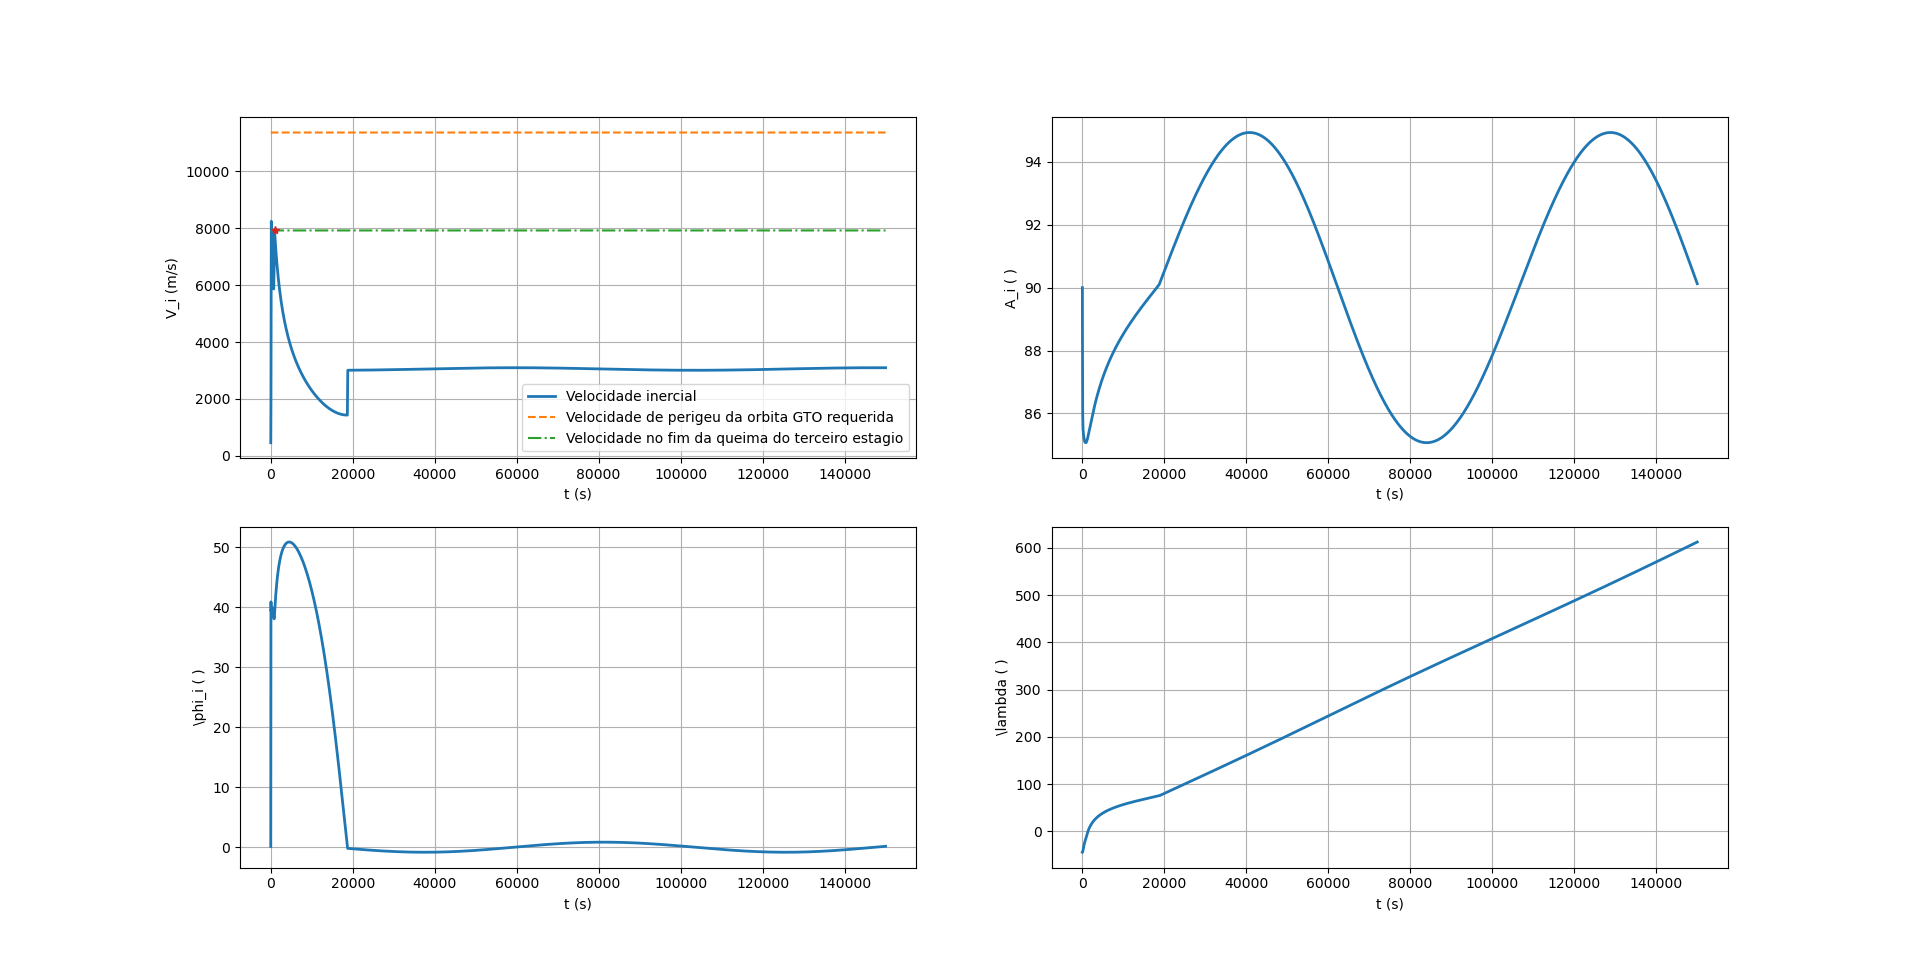
\includegraphics[width=6in]{figuras/Figure_2.png}
        \label{fig:3}
      \fonte{Autores.}
     \end{center}
\end{figure}

É interessante notar que a velocidade de perigeu da órbita GTO requerida não foi atingida, porém a velocidade foi suficiente para a inserção em órbita GSO. Além disso, o ângulo do Azimute varia muito durante o lançamento. 

\begin{figure}[H]
    \begin{center}
        \caption{Variáveis atmosféricas.}
        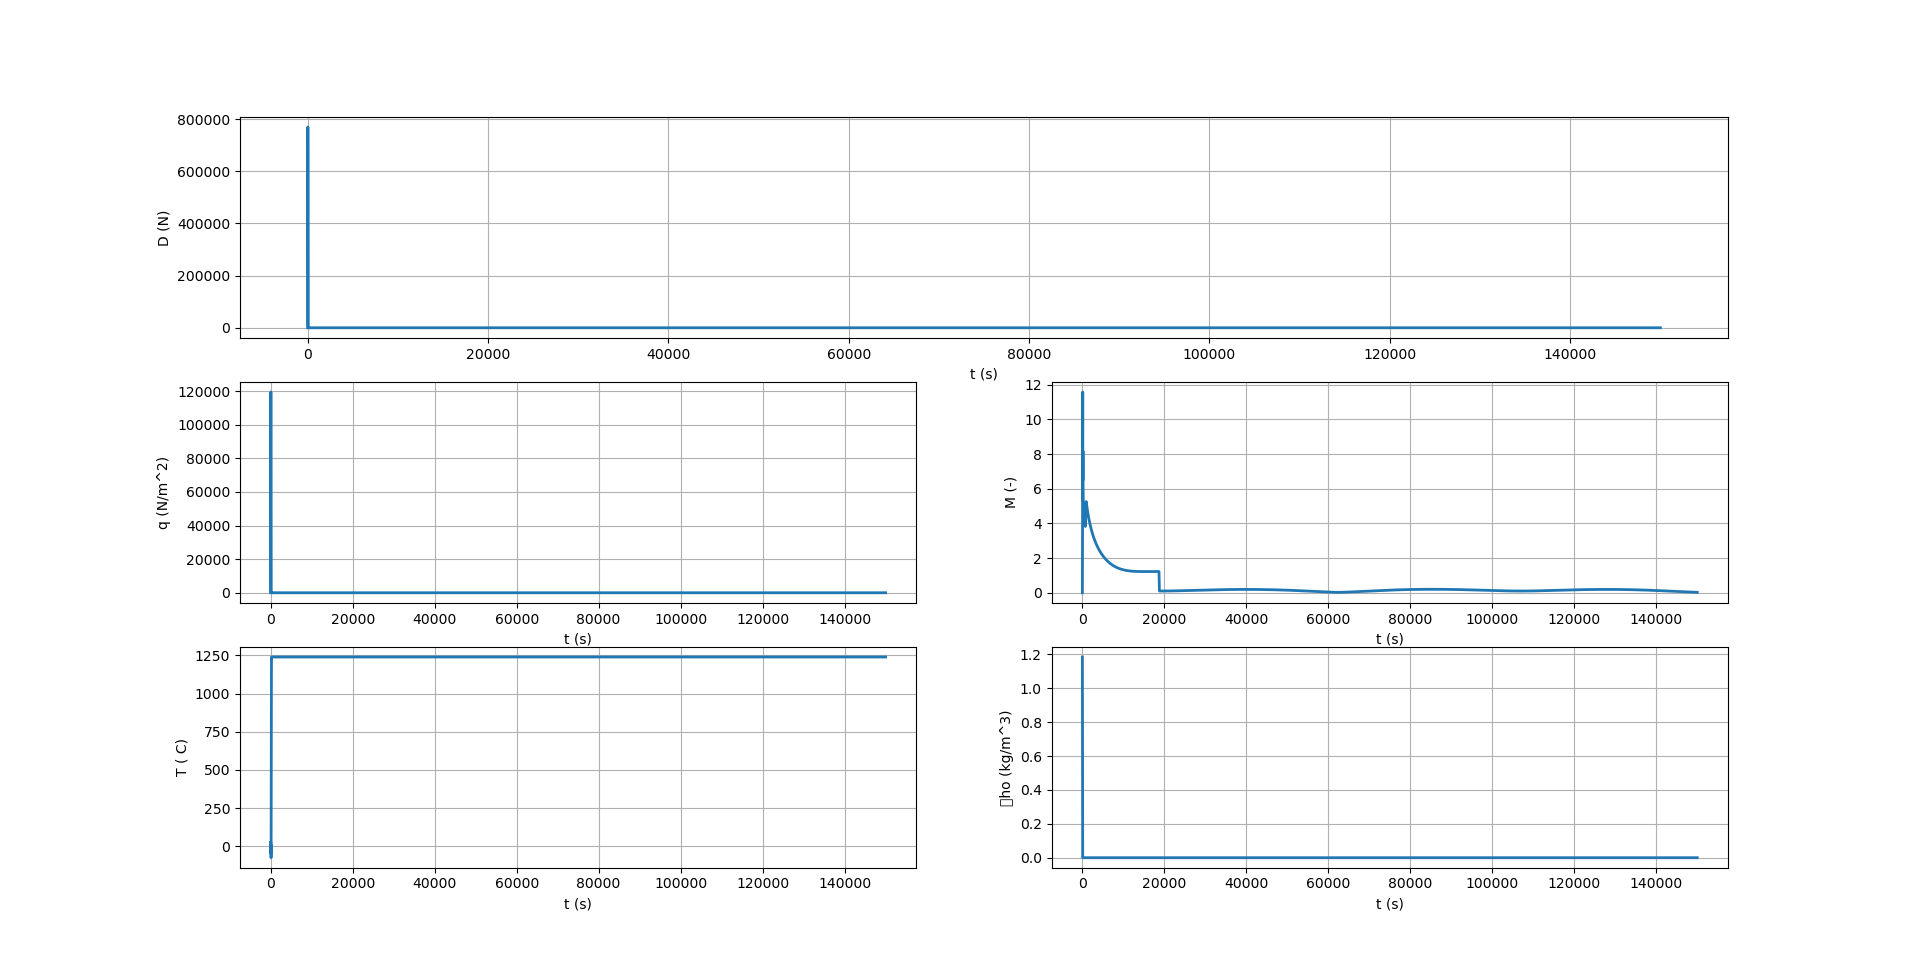
\includegraphics[width=6in]{figuras/Figure_4.png}
        \label{fig:3}
      \fonte{Autores.}
     \end{center}
\end{figure}

Como dito anteriormente, as variáveis atmosféricas influenciam principalmente durante os primeiros instantes do lançamento, após isso, conforma a altitude aumenta, esses feitos tendem a diminuir e influenciar pouco. Além disso, para a inserção em órbita GSO, é necessário levar o foguete até um pouco em que o mesmo sofra com baixas forças atmosféricas.

\begin{figure}[H]
    \begin{center}
        \caption{Parâmetros da órbita final.}
        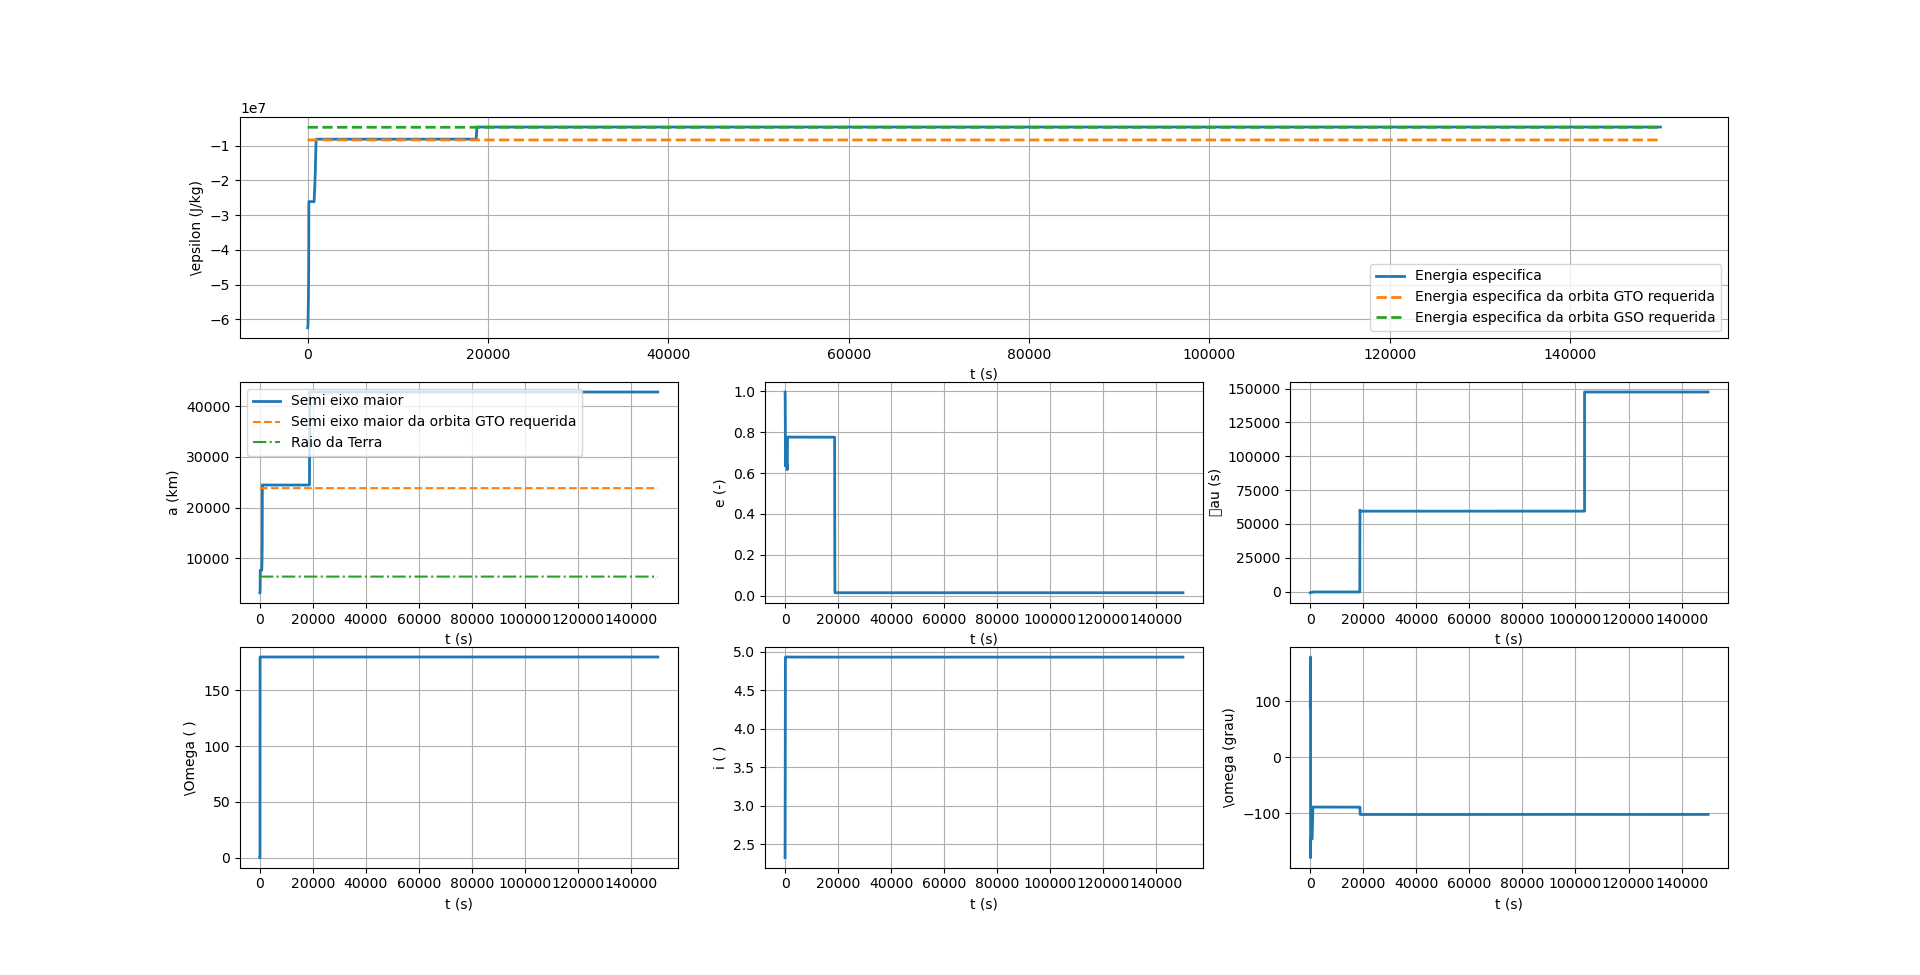
\includegraphics[width=6in]{figuras/Figure_5.png}
        \label{fig:3}
      \fonte{Autores.}
     \end{center}
\end{figure}

A energia específica para a órbita geossíncrona foi atingida após a energia específica para a órbita GTO ser atingida, resultando no sucesso da inserção na órbita GSO utilizando múltiplas ignições do motor do último estágio, que foi ignitado duas vezes.

\begin{figure}[H]
    \begin{center}
        \caption{Variáveis durante o lançamento.}
        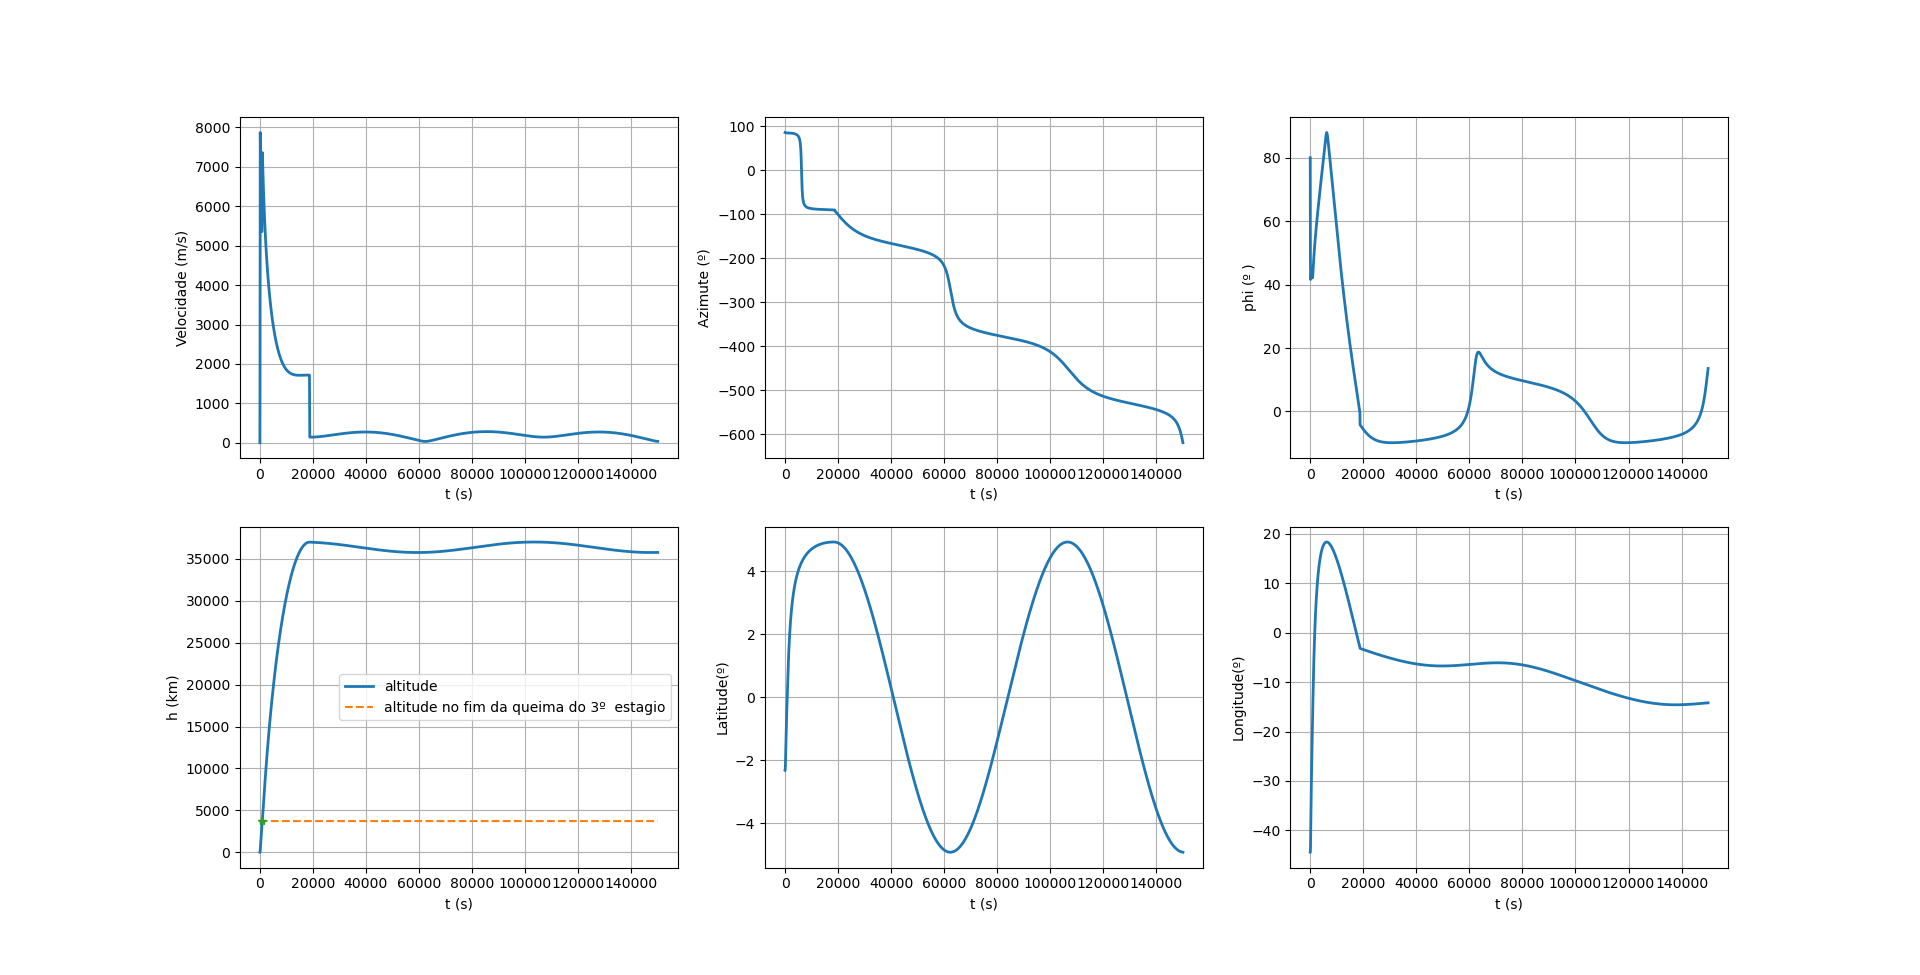
\includegraphics[width=6in]{figuras/Figure_1.png}
        \label{fig:3}
      \fonte{Autores.}
     \end{center}
\end{figure}

A altitude continua aumentando após o fim da queima do terceiro estágio e passa a se estabilizar após a segunda queima do terceiro estágio. A velocidade tem seu pico logo no início do lançamento, sofrendo variação durante a queima do segundo estágio e, por fim, pequenas variações ao longo das queimas do terceiro estágio. Novamente, o Azimute sofre grandes variações, junto da elevação. 

\begin{figure}[H]
    \begin{center}
        \caption{Órbita final atingida pelo veículo.}
        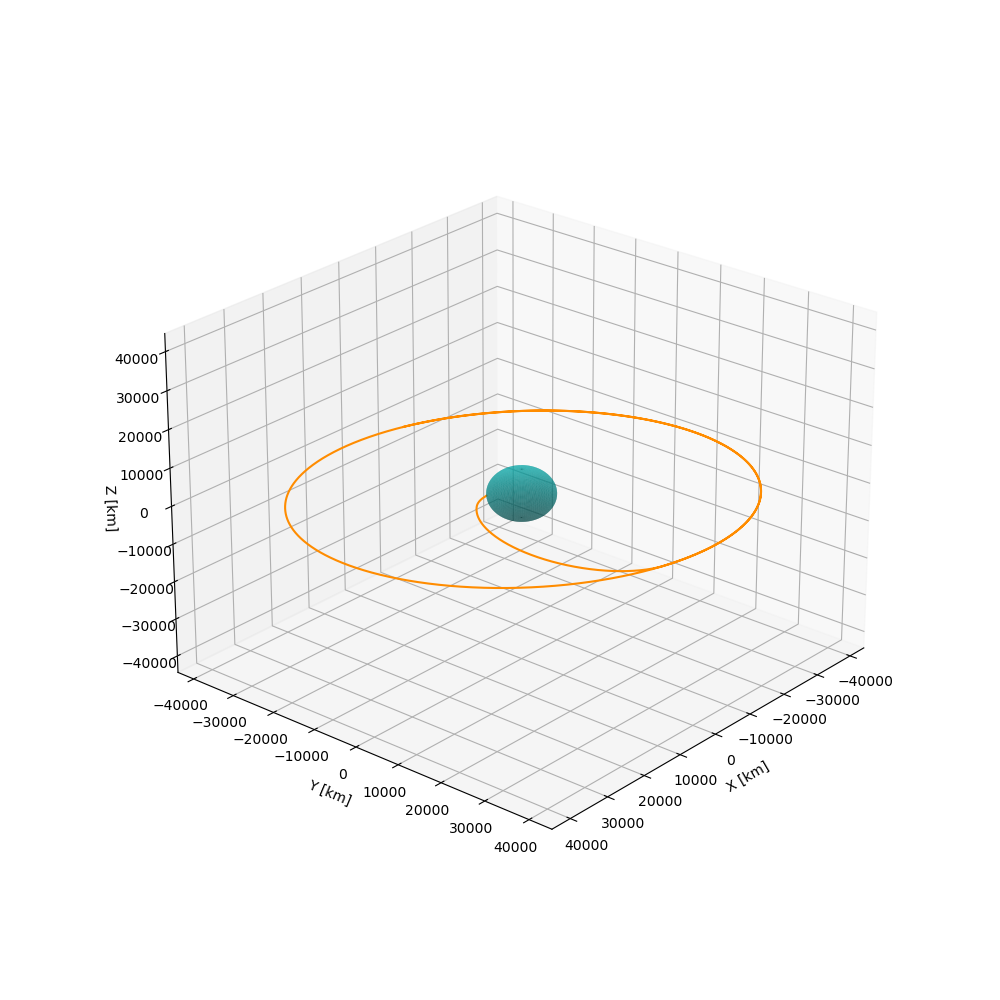
\includegraphics[width=6in]{figuras/fig_6.png}
        \label{fig:3}
      \fonte{Autores.}
     \end{center}
\end{figure}

É possível notar que a órbita geossíncrona foi atingida utilizando os dados descritos anteriormente utilizando praticamente toda a massa de propelente disponível. É visto que a excentricidade é quase nula, sendo um requisito para órbitas geossíncronas. 

\par No gráficos gráficos abaixo, fica claro que a maior energia é utilizada durante os primeiros minutos da missão, sendo essa necessária para "vencer" a força do campo gravitacional terrestre e o arrasto atmosférico. Isso é percebido pelo picos de força propulsiva e do arrasto. 
\begin{figure}[H]
    \begin{center}
        \caption{Valores atingidos durante a queima.}
        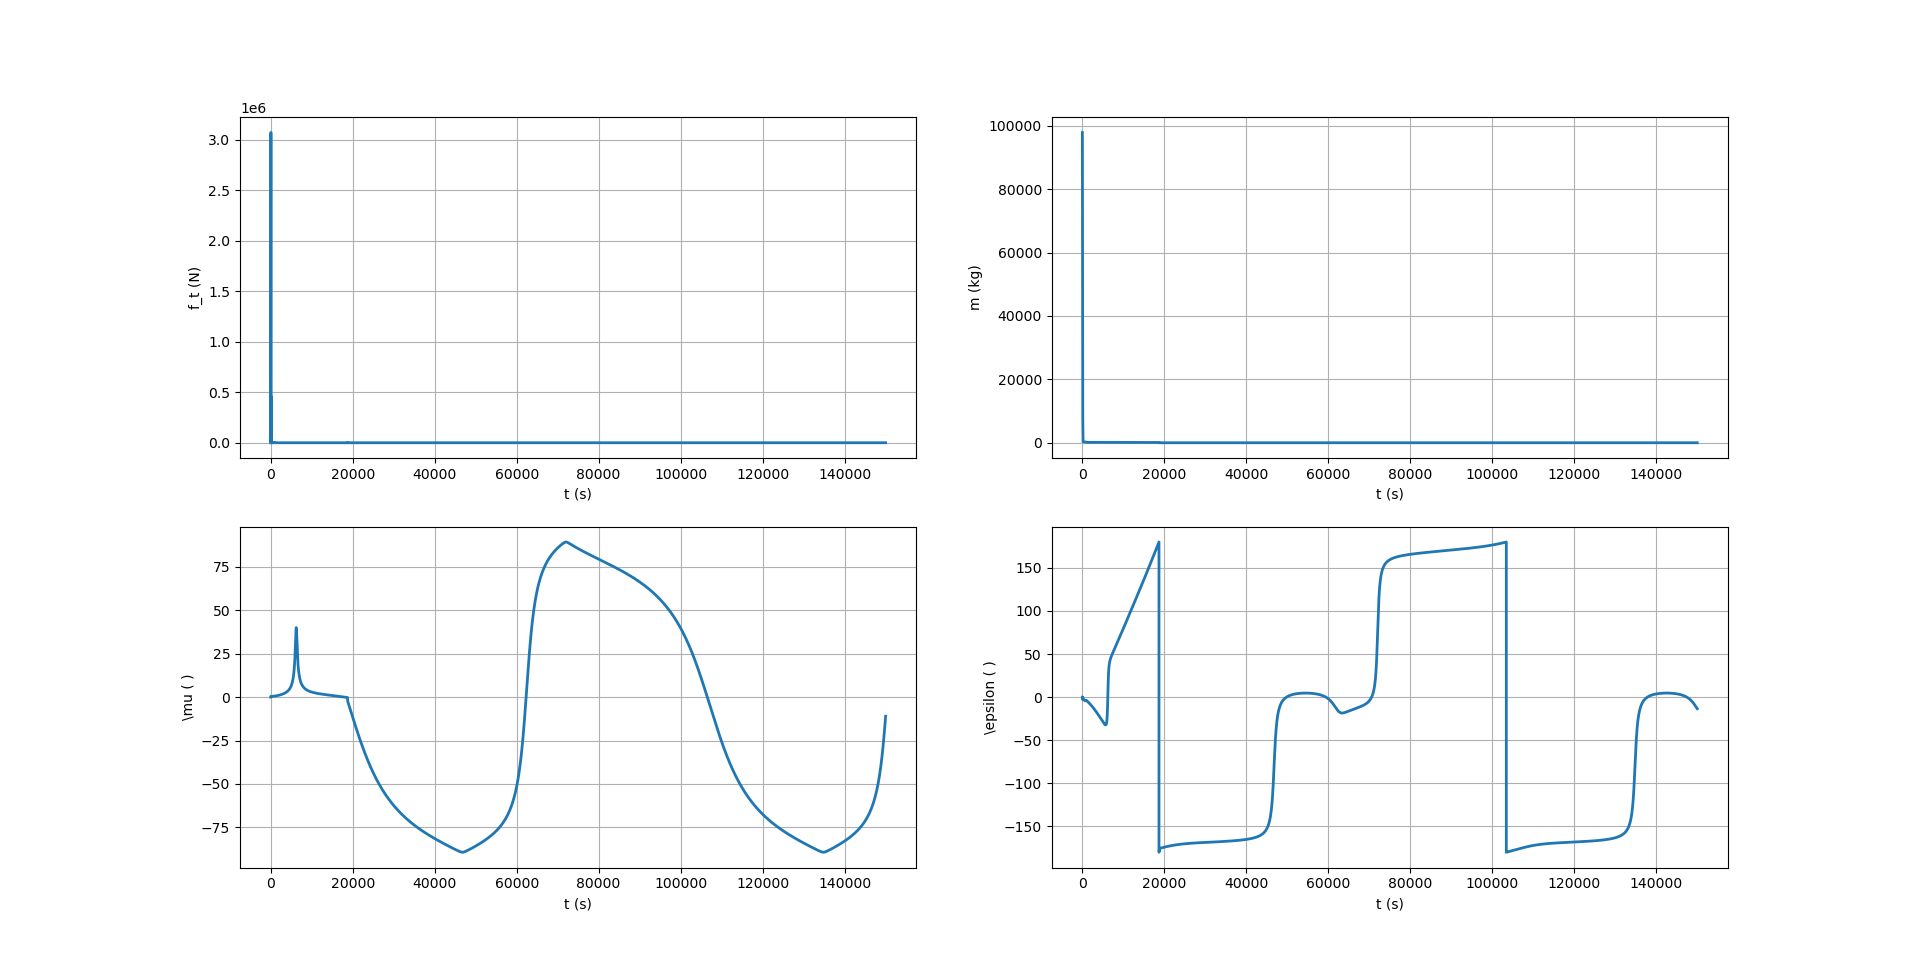
\includegraphics[width=6in]{figuras/Figure_3.png}
        \label{fig:3}
      \fonte{Autores.}
     \end{center}
\end{figure}


\chapter{Conclusão}
\input{Texto/Conclusão}
\chapter{Trabalhos futuros}

Pesquisas futuras poderiam concentrar-se na modulação da direção dos foguetes, especificamente no controle do apontamento do bocal propulsor. Uma estratégia promissora seria o desenvolvimento de um algoritmo de controle inovador, cuja eficácia seria avaliada sob uma variedade de condições de voo. Adicionalmente, a análise do controle das superfícies de empenagem de foguetes poderia desempenhar um papel crucial na otimização da dinâmica de voo. Tal investigação tem o potencial de incrementar a estabilidade e a eficiência do voo do foguete, contribuindo para avanços significativos nesta área. Para uma avaliação mais fidedigna do comportamento dos foguetes em voo, sugere-se a utilização de dados oriundos de lançamentos reais, ao invés da aplicação exclusiva de estimativas teóricas. Essa metodologia ofereceria uma visão mais autêntica do desempenho do foguete em condições reais de voo. Outra linha de investigação poderia contemplar a alteração do design do foguete e a distribuição de massa no seu interior. Isso poderia incluir a modificação da forma do foguete ou a reconsideração da quantidade e disposição do combustível. Essas mudanças poderiam levar a melhorias significativas no desempenho dos foguetes.
\input{Texto/Conclusão}
	
	
% % % % % % % % % % % % % % % % % % % % % % % % % % % % % % % % % % % % % % 
% % % % % % % % % % % % FIM DAS PAGINAS TEXTUAIS % % % % % % % % % % % % % % 
% % % % % % % % % % % % % % % % % % % % % % % % % % % % % % % % % % % % % % 



% % % % % % % % % % % % % % % % % % % % % % % % % % % % % % % % % % % % % % 	
% % % % % % % % % % % % % BIBLIOGRAFIA  % % % % % % % % % % % % % % % % % % 
% % % % % % % % % % % % % % % % % % % % % % % % % % % % % % % % % % % % % % 	

\startbibliography % comando para formatar na MDT UFSM
\bibliography{referencias}

	
% % % % % % % % % % % % % % % % % % % % % % % % % % % % % % % % % % % % % 	
% % % % % % % % % % % % % APENDICES % % % % % % % % % % % % % % % % % % %
% % % % % % % % % % % % % % % % % % % % % % % % % % % % % % % % % % % % % 	
\apendice %%%% TEXTOS A PARIR DESTE PONTO SERAO CONSIDERADOS APENDICES

\end{document}
